\documentclass{acmsiggraph}

\usepackage[utf8]{inputenc}
\usepackage[T1]{fontenc}
\usepackage{graphicx}
\usepackage{amsmath}
\usepackage{booktabs}
\usepackage{subcaption}

\title{Running Data Accuracy: Comparing Upper-Arm Sensors and Smartwatches}

\author{Volkan Korunan\\Berliner Hochschule f\"ur Technik, Matrikel-Nr. 824145}
\pdfauthor{Volkan Korunan}

\keywords{wearable sensors, heart rate monitoring, PPG, GPS tracking, sensor validation}

\setcopyright{rightsretained}
\copyrightyear{2026}
\conferenceinfo{Wissenschaftliches Arbeiten}{SoSe 2026, Berliner Hochschule f\"ur Technik}

\begin{document}
	
	\maketitle
	
	\begin{abstract}
		The accurate tracking of heart rate (HR) and geospatial data during sports
		activities is crucial for reliable performance analysis. Although
		wrist-worn smartwatches are considered the consumer standard, physical
		motion artifacts often compromise data integrity. This paper compares the
		data continuity and cross-device agreement of a wrist-worn smartwatch
		(Amazfit GTR~3~Pro) and an optical upper-arm sensor (Coospo~HW9) during
		outdoor running. Because both devices are consumer-grade and neither is a
		clinically validated reference (e.g., an ECG chest strap), our results
		describe \emph{agreement between two consumer sensors} rather than
		absolute accuracy against ground truth. Based on a synchronized field
		study ($N=6$ trials with a single runner), average per-run HR means align
		closely between devices, but instantaneous agreement is more variable:
		aggregated across all six runs, mean Pearson $r=0.60$ (median $0.66$),
		mean MAE $=8.9$\,bpm, and mean bias $=+4.6$\,bpm. Geospatial tracks agree
		reasonably well overall (mean $\Delta$GPS~$\approx$~4.56\,m across all
		six runs, ranging from 2.1 to 8.3\,m per-run mean, max.\ 30.5\,m; mean
		track-length error $\approx$~1.5\%, range 0.5--4.2\%). Speed agreement
		falls between these two: mean Pearson $r=0.73$ (median $0.75$) and mean
		MAE $=1.09$\,km/h across all six runs. The wrist-worn device shows
		substantial signal dropouts, missing heart rate data for up to 74.6\% of
		a run's duration and failing to register several transient cardiac load
		peaks. A post-hoc power analysis indicates that $n\approx13$ trials would
		be required for a conventionally powered validation; at $N=6$ trials from
		a single subject, this study reaches only 53.2\% of that target and
		should be read as an underpowered, exploratory pilot rather than a
		confirmatory validation. We further note that the two devices differ not
		only in sensor placement but also in hardware generation and physical
		condition, so placement effects cannot be cleanly separated from these
		confounds in the present design.
	\end{abstract}
	
	% ---------------------------------------------------------------
	\section{Introduction}
	
	Wearable fitness trackers have democratized performance diagnostics for
	recreational and professional athletes alike. For runners, real-time
	heart rate (HR) monitoring serves as a primary metric for training
	intensity distribution and metabolic threshold management. However, the
	commercial market is split between different form factors and sensor
	placements.
	
	Wrist-worn smartwatches leverage photoplethysmography (PPG) to measure
	blood volume changes through the skin \cite{kim_photoplethysmography_2023}. While highly
	convenient, this placement is notoriously susceptible to motion-induced
	artifacts caused by rhythmic arm swings, gripping forces, and rapid
	cadence shifts during running \cite{kim_photoplethysmography_2023,schweizer2024heart}. These
	artifacts introduce high-frequency noise, often leading to signal loss
	or algorithmic miscalculations. Alternatively, upper-arm mounted sensors
	present a promising compromise, placing the optical array on a larger
	muscular surface (e.g., biceps brachii) with less dynamic independent
	movement \cite{schweizer2024heart}.
	
	This paper compares the tracking behavior, signal reliability, and
	geospatial mapping of a wrist-worn smartwatch and an upper-arm mounted
	sensor. Because the upper-arm device is itself a consumer sensor rather
	than a validated reference standard, we frame our contribution as a
	quantification of \emph{cross-device agreement and data density}, not as
	an absolute accuracy assessment. By evaluating data density, velocity
	profiles, and peak-value detection across a synchronized field study, we
	document the operational limitations of the wrist-based device under the
	conditions tested here.
	
	% ---------------------------------------------------------------
	\section{State of the Art}
	
	Validation studies for consumer wearables generally fall into two
	categories: controlled laboratory environments using treadmill protocols,
	and free-living field tests. Wearable GPS-enabled sport watches and
	smartphones are now widely adopted among amateur athletes for tracking
	and optimizing training \cite{pobiruchin2017accuracy}.
	
	\subsection{Wrist-Based PPG Limitations}
	
	Prior research indicates that wrist-worn devices demonstrate acceptable
	accuracy during low-motion states (e.g., cycling or walking). Commercial
	wearables are generally accurate for measuring heart rate in laboratory
	settings, with devices from established brands performing best
	\cite{fuller_reliability_2020}. However, none of the wrist-worn devices tested in
	these reviews have proven accurate for measuring energy expenditure
	\cite{fuller_reliability_2020,germini_accuracy_2022}. The mechanical displacement of the watch
	body creates transient air gaps between the photodiode and the skin,
	causing ambient light leakage \cite{kim_photoplethysmography_2023}. Although green light is
	widely used in wearable PPG for its absorption characteristics, it
	remains vulnerable to motion artifacts during vigorous activity
	\cite{kim_photoplethysmography_2023}. During triathlon training, wrist smartwatches have been
	shown to exhibit mean absolute percentage errors for heart rate between
	3.1\% and 8.3\%, with distance-tracking accuracy dropping further during
	complex motion \cite{jacko_validity_2024}.
	
	\subsection{Alternative Sensor Placements}
	
	To mitigate these limitations, sports science literature has explored
	alternative body sites. Optical sensors worn on the forearm or upper arm
	benefit from a more stable tissue mass with less independent motion.
	Analytical validation studies show that upper-arm optical sensors exhibit
	good validity and reliability, whereas wrist-worn devices show accuracy
	that varies strongly with the level of motion artifact
	\cite{schweizer2024heart}. It should be noted that such comparisons, including
	our own, typically evaluate agreement between two consumer-grade devices
	rather than accuracy against a clinical reference such as an
	electrocardiogram (ECG) chest strap.
	
	% ---------------------------------------------------------------
	\section{Methodology}
	
	To evaluate the systematic differences between the two tracking
	topologies, a synchronized field testing protocol was established. The
	study was conducted on an asphalted outdoor route characterized by a
	dense tree canopy, providing a challenging environment for
	satellite-based navigation.
	
	\subsection{Hardware Configuration}
	
	Two distinct commercial optical devices were worn simultaneously by the
	same subject:
	\begin{itemize}
		\item \textbf{Wrist Device (HG):} Amazfit GTR~3~Pro with a BioTracker
		PPG~3.0 sensor, sampling at a nominal frequency of 1\,Hz. This device
		had an operational lifespan exceeding four years at the time of
		testing, with visible mechanical degradation of the optical sensor
		window (discussed in Section~5).
		\item \textbf{Upper-Arm Device (OA):} Coospo~HW9 optical heart rate
		sensor, attached via an elastic band to the dominant biceps brachii and
		streaming via Bluetooth LE. This device was newer, both in hardware
		generation and physical condition.
	\end{itemize}
	Because the two devices differ simultaneously in sensor placement,
	hardware generation, and physical wear, placement effects cannot be
	isolated from these confounds in the present design; we return to this
	limitation in Section~5.
	
	\subsection{Data Acquisition \& Processing}
	
	The evaluation uses a data matrix comprising $N=6$ distinct outdoor
	running trials, each a single continuous run along the same route,
	performed by the same subject on separate occasions. An intra-subject
	design was chosen to eliminate inter-subject demographic confounders.
	For data synchronization, timestamps from both devices were independently
	rounded to the nearest full second and joined via an inner merge on this
	common 1-second key, so that only strictly overlapping, mutually valid
	samples contributed to the comparison; the resulting synchronized
	duration corresponds to the intersection of both devices' recording
	windows. A structural anomaly discovered during preprocessing concerned
	heart rate data density: while the upper-arm sensor recorded continuous
	telemetry across all six trials, the smartwatch produced substantial
	gaps in 4 of the 6 runs, dropping up to 74.6\% of cardiac data points,
	likely attributable to a combination of motion-induced artifacts and the
	sensor degradation described in Section~5.
	
	% ---------------------------------------------------------------
	\section{Results}
	
	The empirical analysis highlights a contrast in signal stability rather
	than a large deviation in baseline geospatial tracks. As compiled in
	Table~\ref{tab:results}, mean heart rate calculated across stable
	intervals is congruent between devices, but severe dropouts limit the
	practical utility of the wrist sensor's data. As visualized in
	Figure~\ref{fig:trend}, the upper-arm sensor (blue) reacts immediately to
	cardiac micro-intensities, whereas the wrist sensor (orange) exhibits a
	smoothing lag and substantial data omissions.
	
	\begin{figure}[!htb]
		\centering
		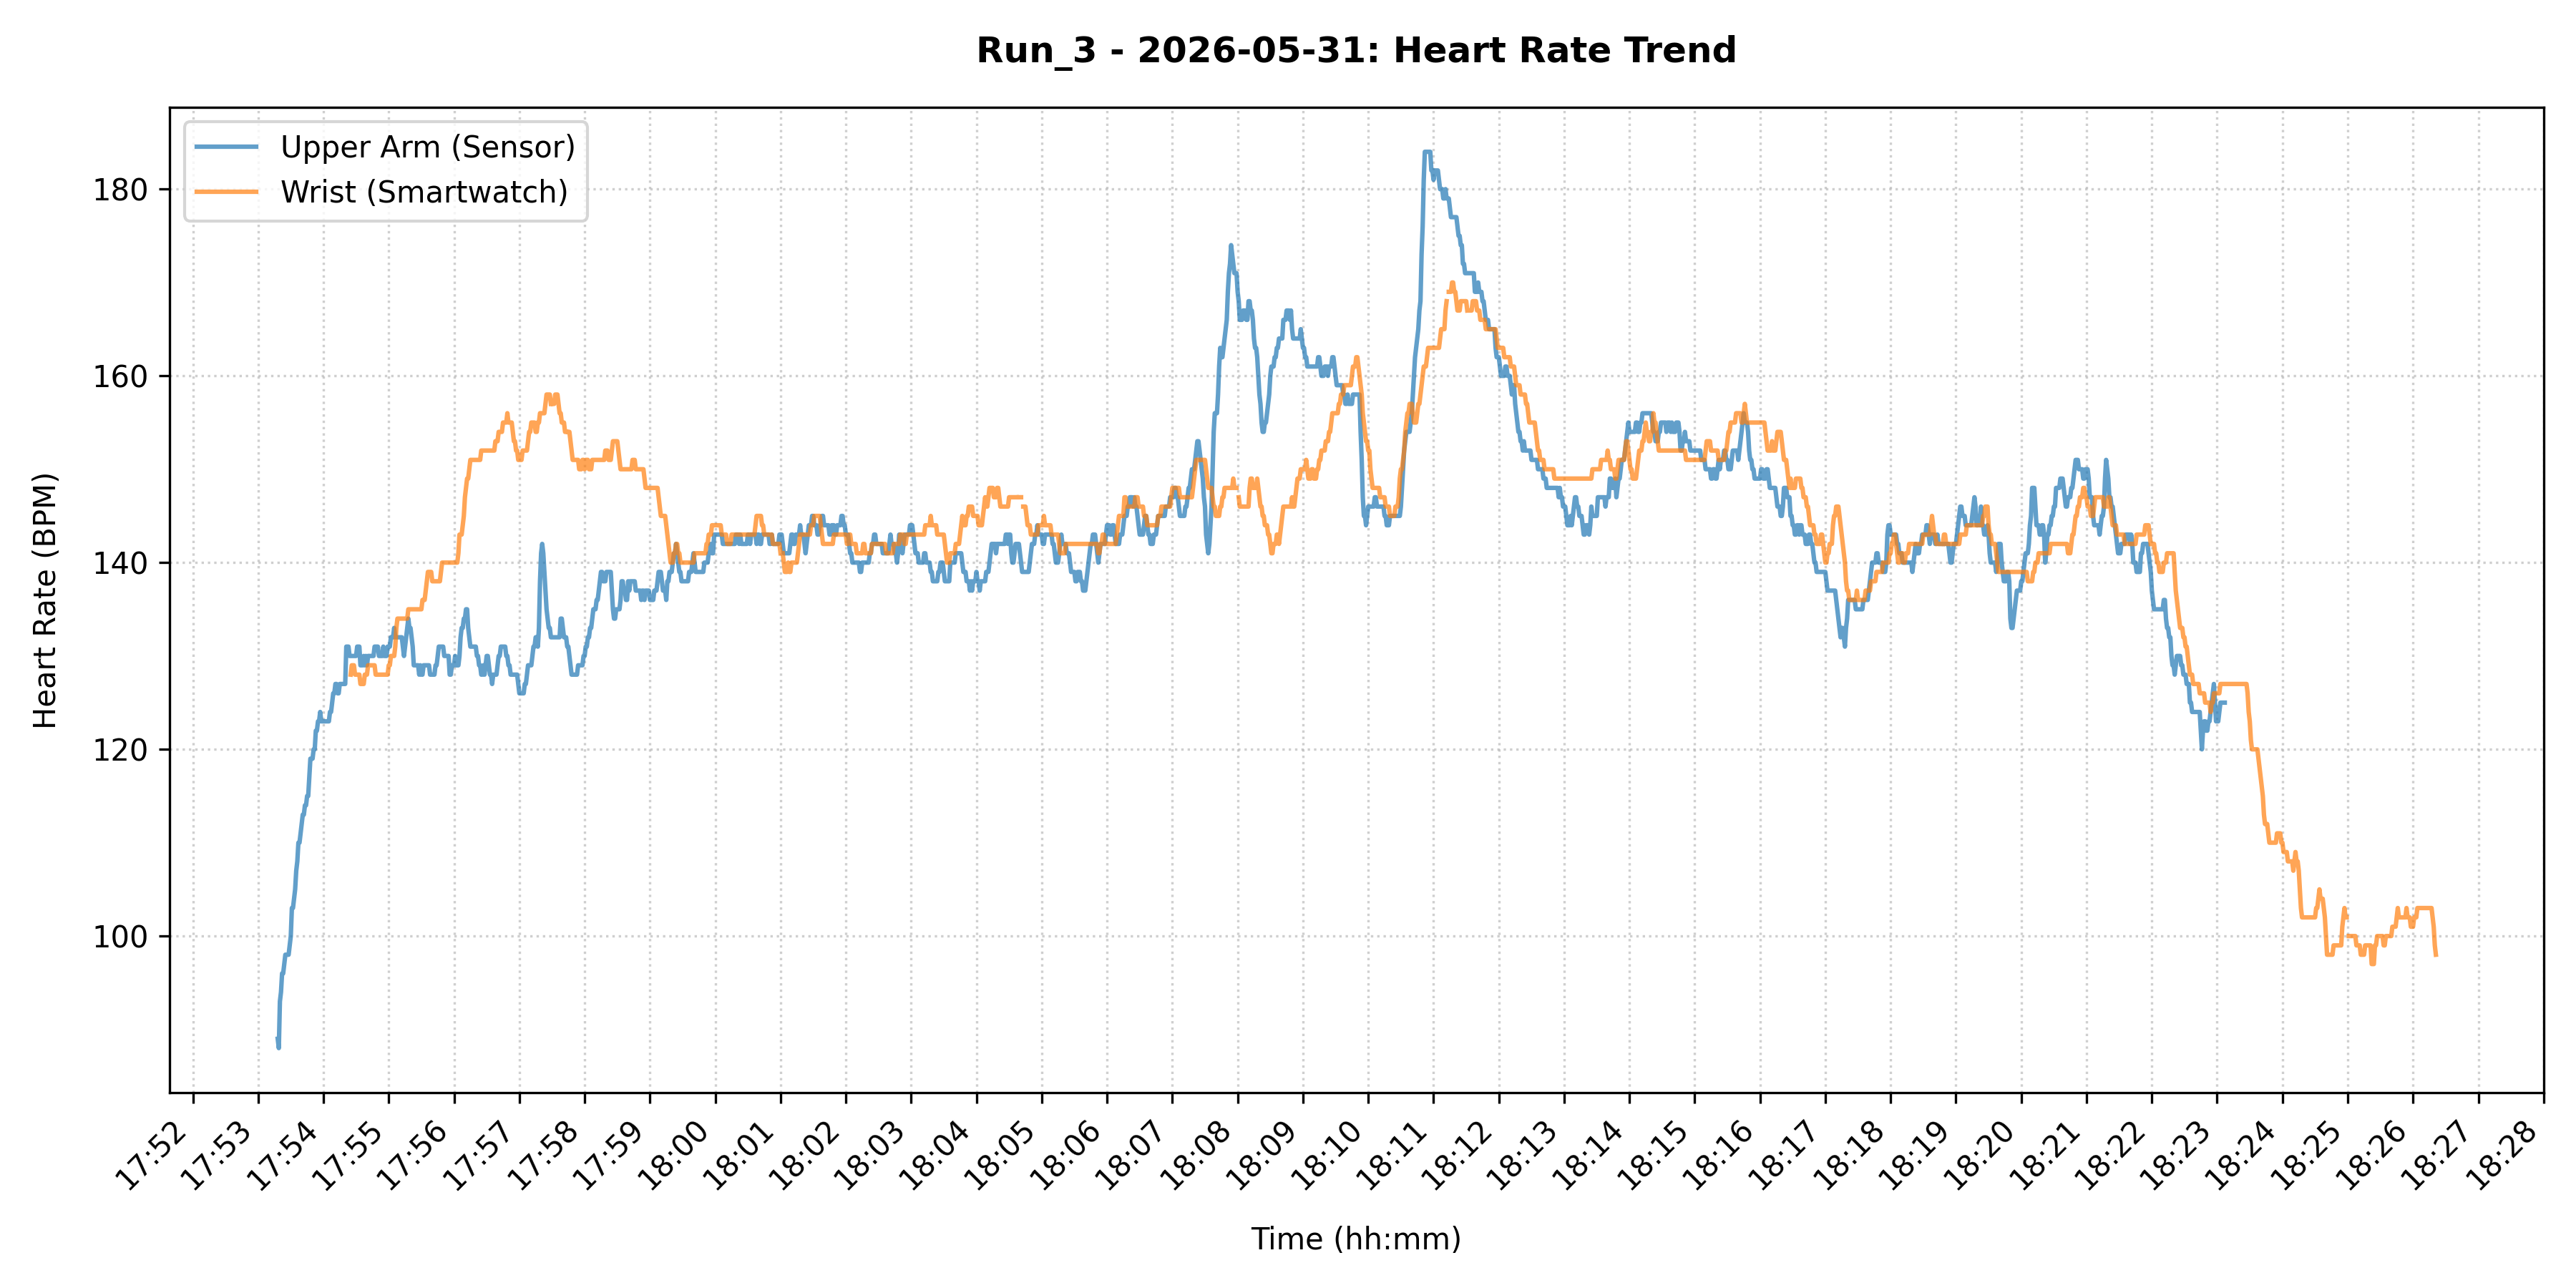
\includegraphics[width=0.9\linewidth]{Run_3_HR_Trend.png}\par\vspace{2mm}
		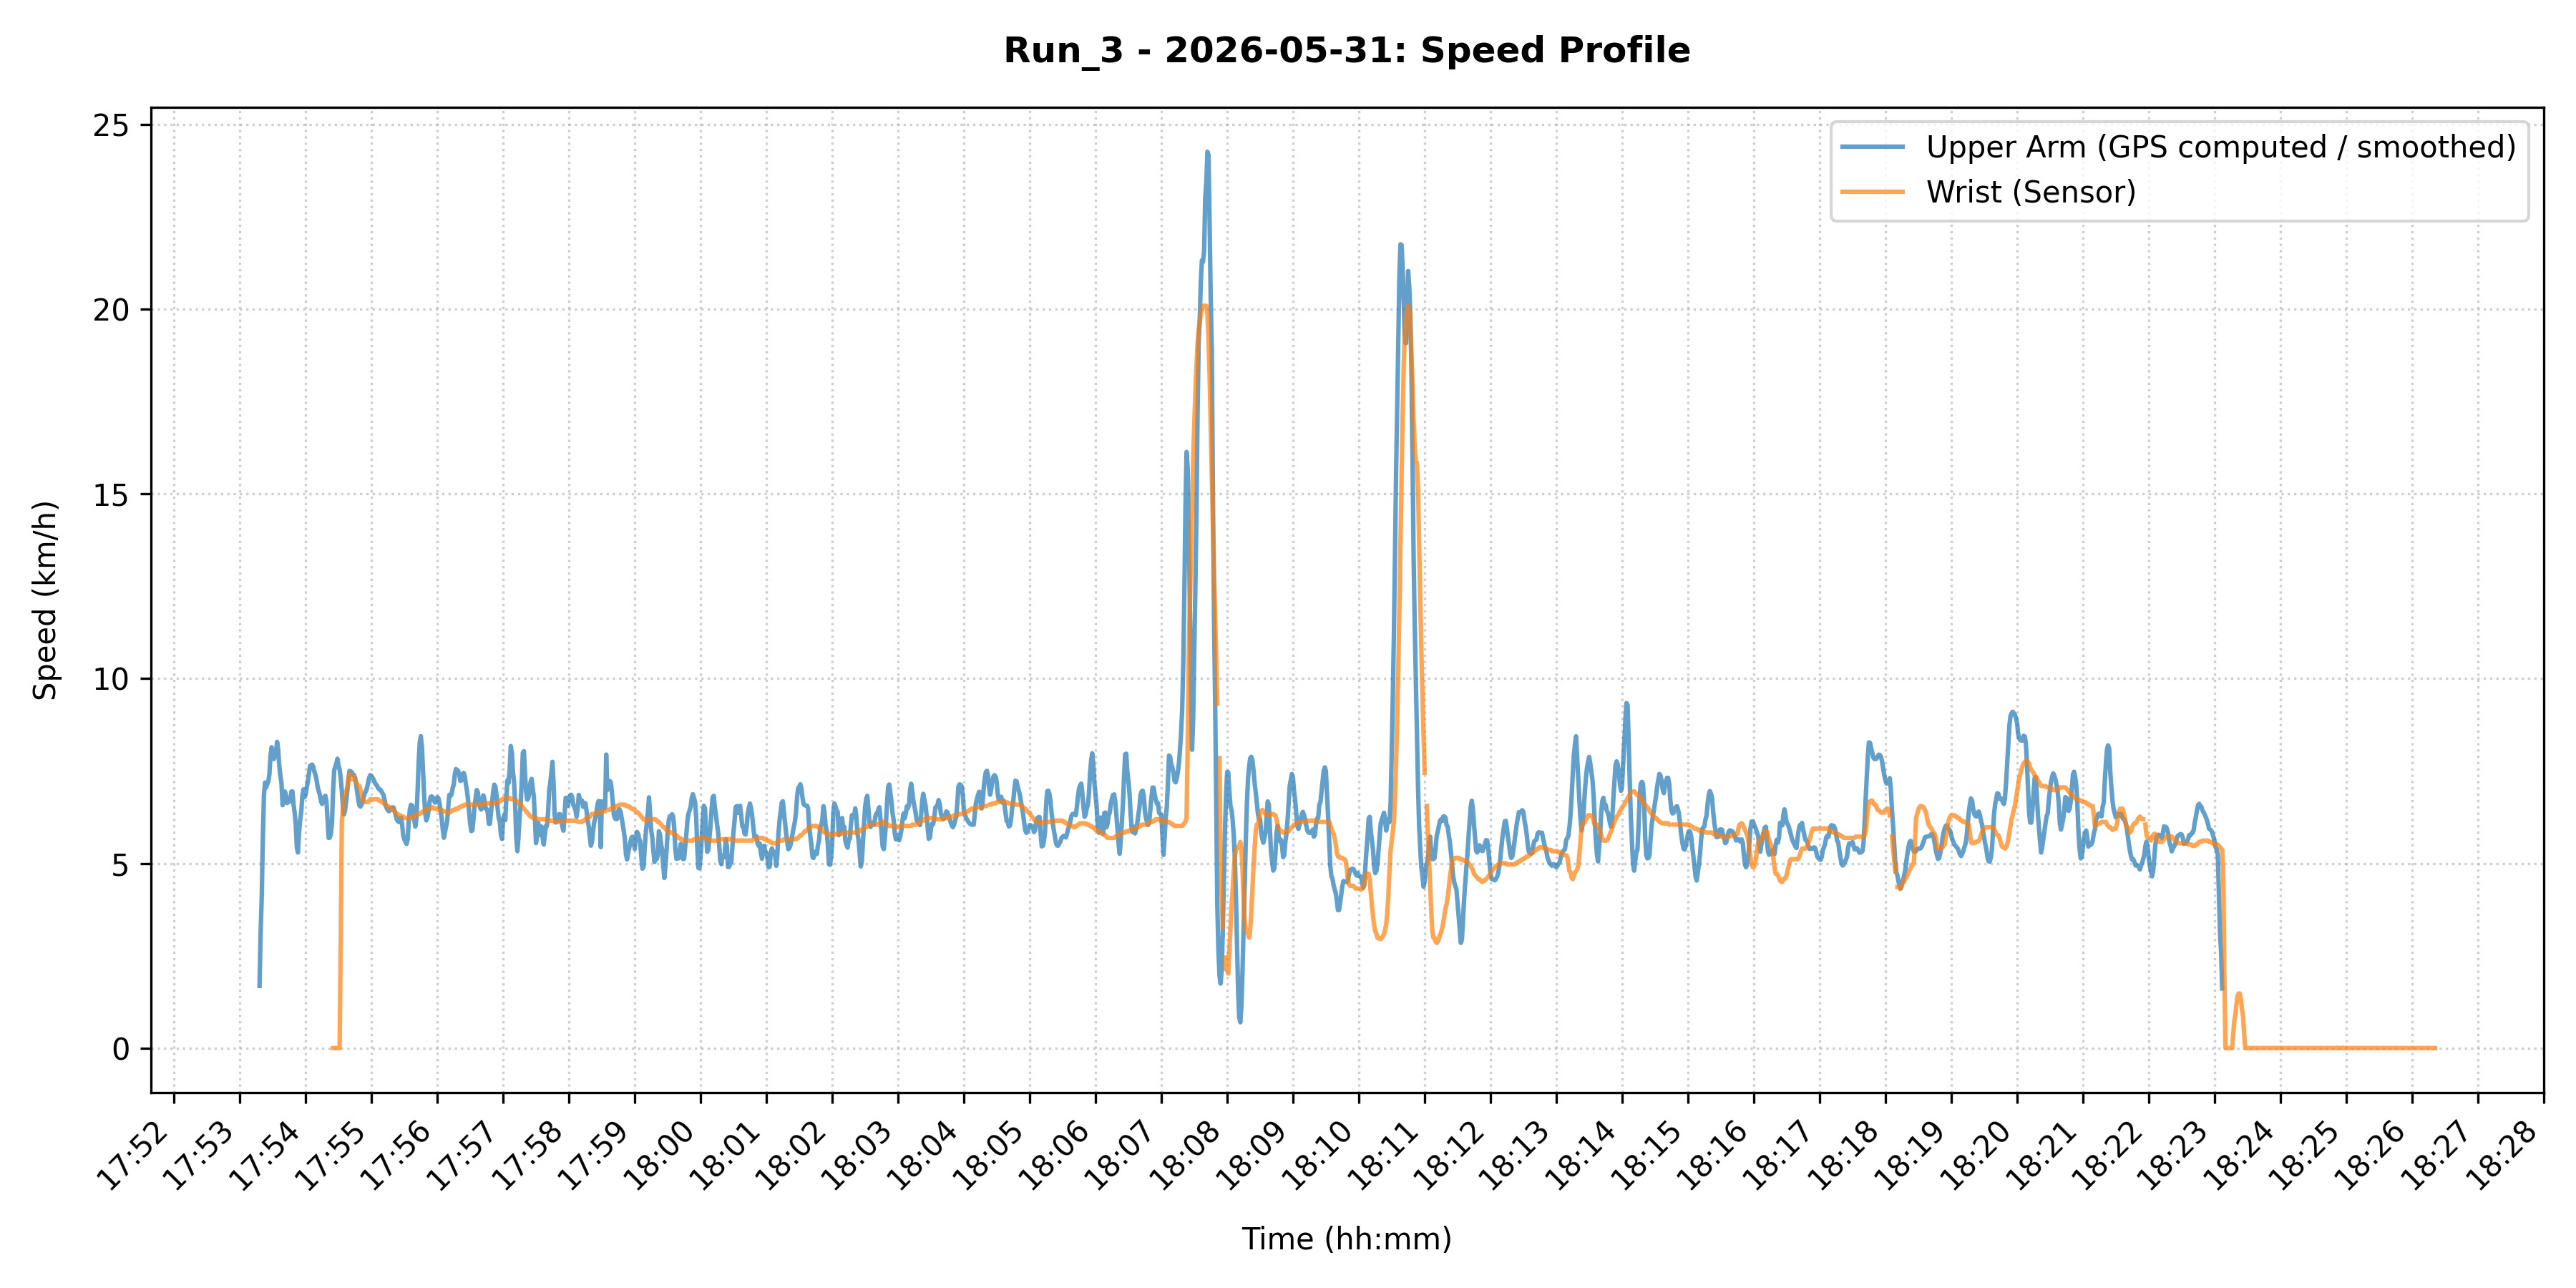
\includegraphics[width=0.9\linewidth]{Run_3_Speed_Profile.png}
		\caption{Comparison of heart rate kinetics (top) and velocity
			profiles (bottom) during Trial 3. The upper-arm sensor (blue) captures
			dynamic peaks, whereas the wrist sensor (orange) exhibits latency and
			data omissions.}
		\label{fig:trend}
	\end{figure}
	
	\begin{table*}[t]
		\centering
		\caption{Comprehensive sensor and track evaluation ($N=6$ synchronized runs).}
		\label{tab:results}
		\small
		\begin{tabular}{lccccccc}
			\toprule
			Metric / Trial & Run 1 & Run 2 & Run 3 & Run 4 & Run 5 & Run 6 & Avg. \\
			\midrule
			Synchronized Duration (s) & 1634.0 & 1556.0 & 1722.0 & 1762.0 & 1617.0 & 1608.0 & 1649.8 \\
			OA Distance (km)          & 3.190  & 2.877  & 3.071  & 3.185  & 3.183  & 3.213  & 3.120 \\
			HG Distance (km)          & 3.176  & 2.911  & 3.072  & 3.174  & 3.168  & 3.193  & 3.116 \\
			Distance Error (\%)       & 1.1    & 4.2    & 2.0    & 0.5    & 0.7    & 0.7    & 1.5 \\
			\midrule
			OA HR Mean / Max (bpm)    & 148.9/186 & 150.8/188 & 144.3/184 & 145.8/180 & 142.9/185 & 153.1/185 & 147.6/184.7 \\
			HG HR Mean / Max (bpm)    & 149.6/168 & 130.8/165 & 146.2/170 & 142.6/169 & 144.0/169 & 155.1/175 & 144.7/169.3 \\
			HG HR Data Loss (s)       & 1184   & 29     & 13     & 1269   & 1144   & 1052   & 781.8 \\
			HR Pearson $r$ / MAE (bpm) & 0.83/4.0 & 0.03/22.1 & 0.65/5.5 & 0.60/9.1 & 0.68/7.1 & 0.80/5.3 & 0.60/8.9 \\
			Speed Pearson $r$ / MAE (km/h) & 0.55/1.65 & 0.72/1.34 & 0.77/0.85 & 0.79/0.76 & 0.84/0.64 & 0.72/1.28 & 0.73/1.09 \\
			\midrule
			Mean / Max GPS Offset (m) & 3.42/10.5 & 7.26/30.5 & 8.26/22.9 & 3.83/11.1 & 2.12/6.6 & 2.48/17.9 & 4.56/16.6 \\
			\bottomrule
		\end{tabular}
	\end{table*}
	
	Figure~\ref{fig:agreement} shows scatterplot and Bland-Altman agreement
	for Trial~3 specifically, chosen as an illustrative example; aggregate
	distributional statistics across all six trials are summarized in
	Table~\ref{tab:results} and in the cross-run figures below.
	
	\begin{figure}[!htb]
		\centering
		\begin{subfigure}[b]{0.9\linewidth}
			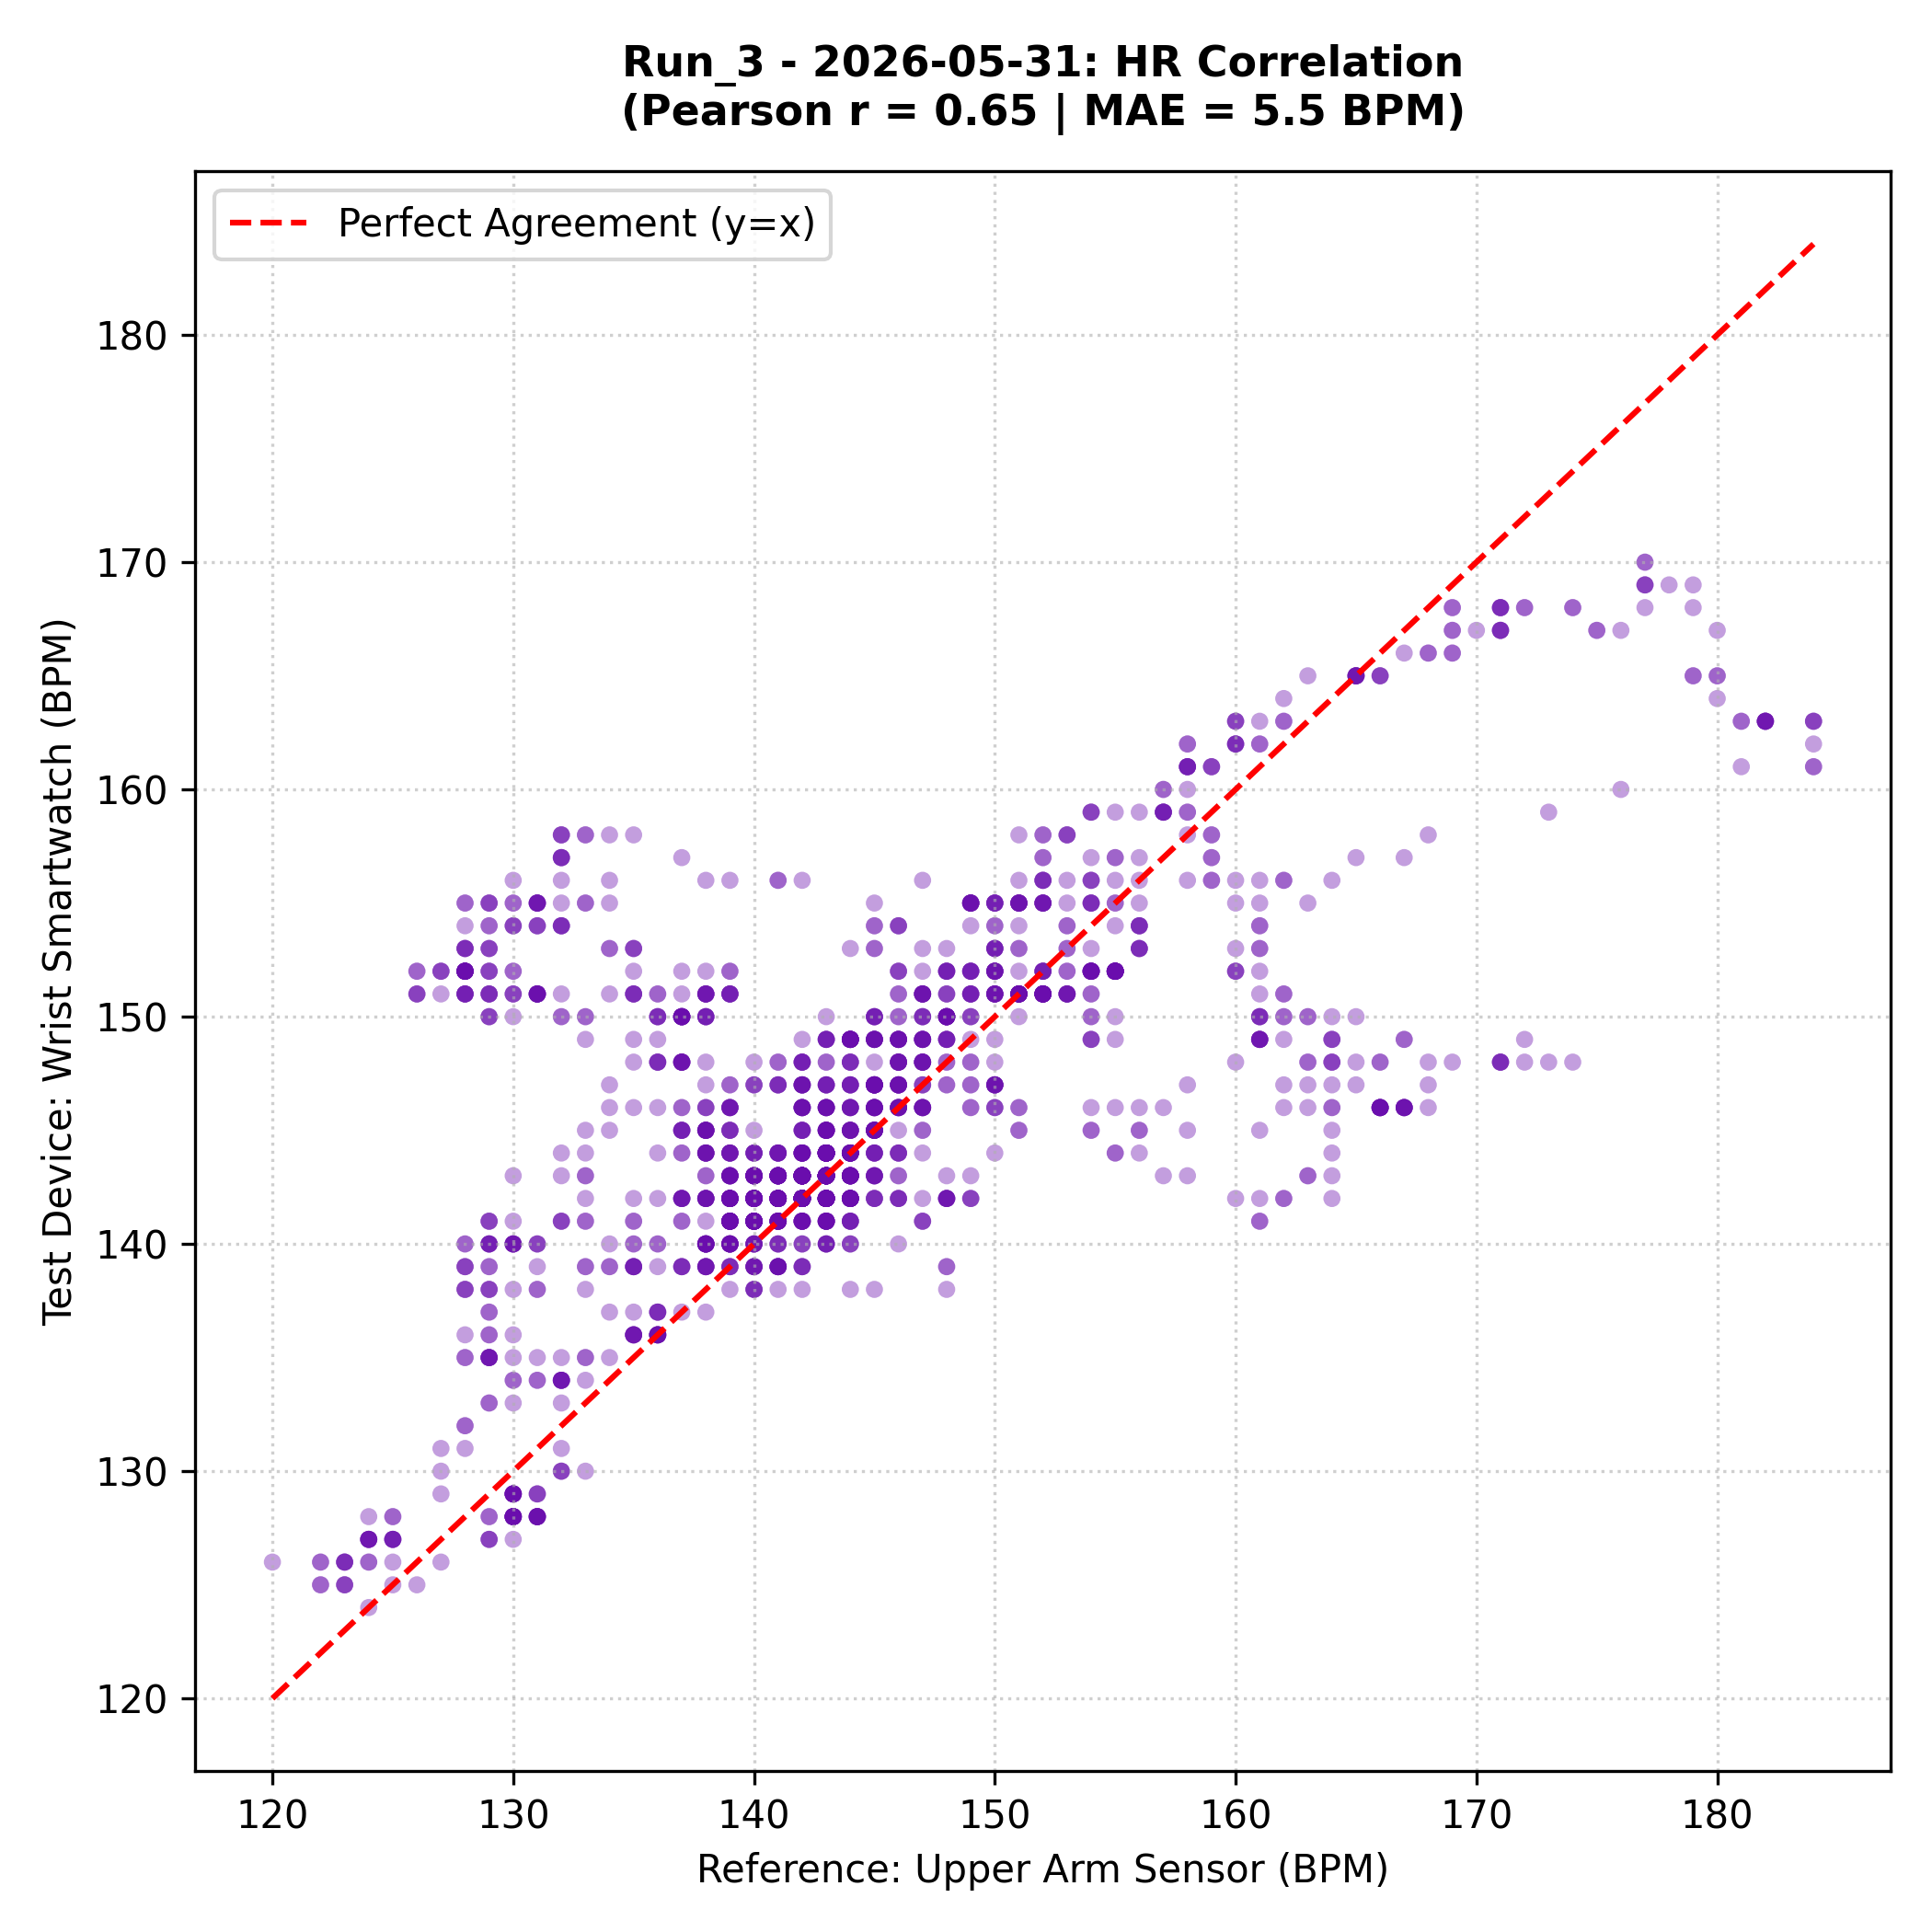
\includegraphics[width=\linewidth]{Run_3_HR_Scatterplot.png}
			\caption{Scatterplot (Trial 3, Pearson $r=0.65$)}
		\end{subfigure}\par\vspace{2mm}
		\begin{subfigure}[b]{0.9\linewidth}
			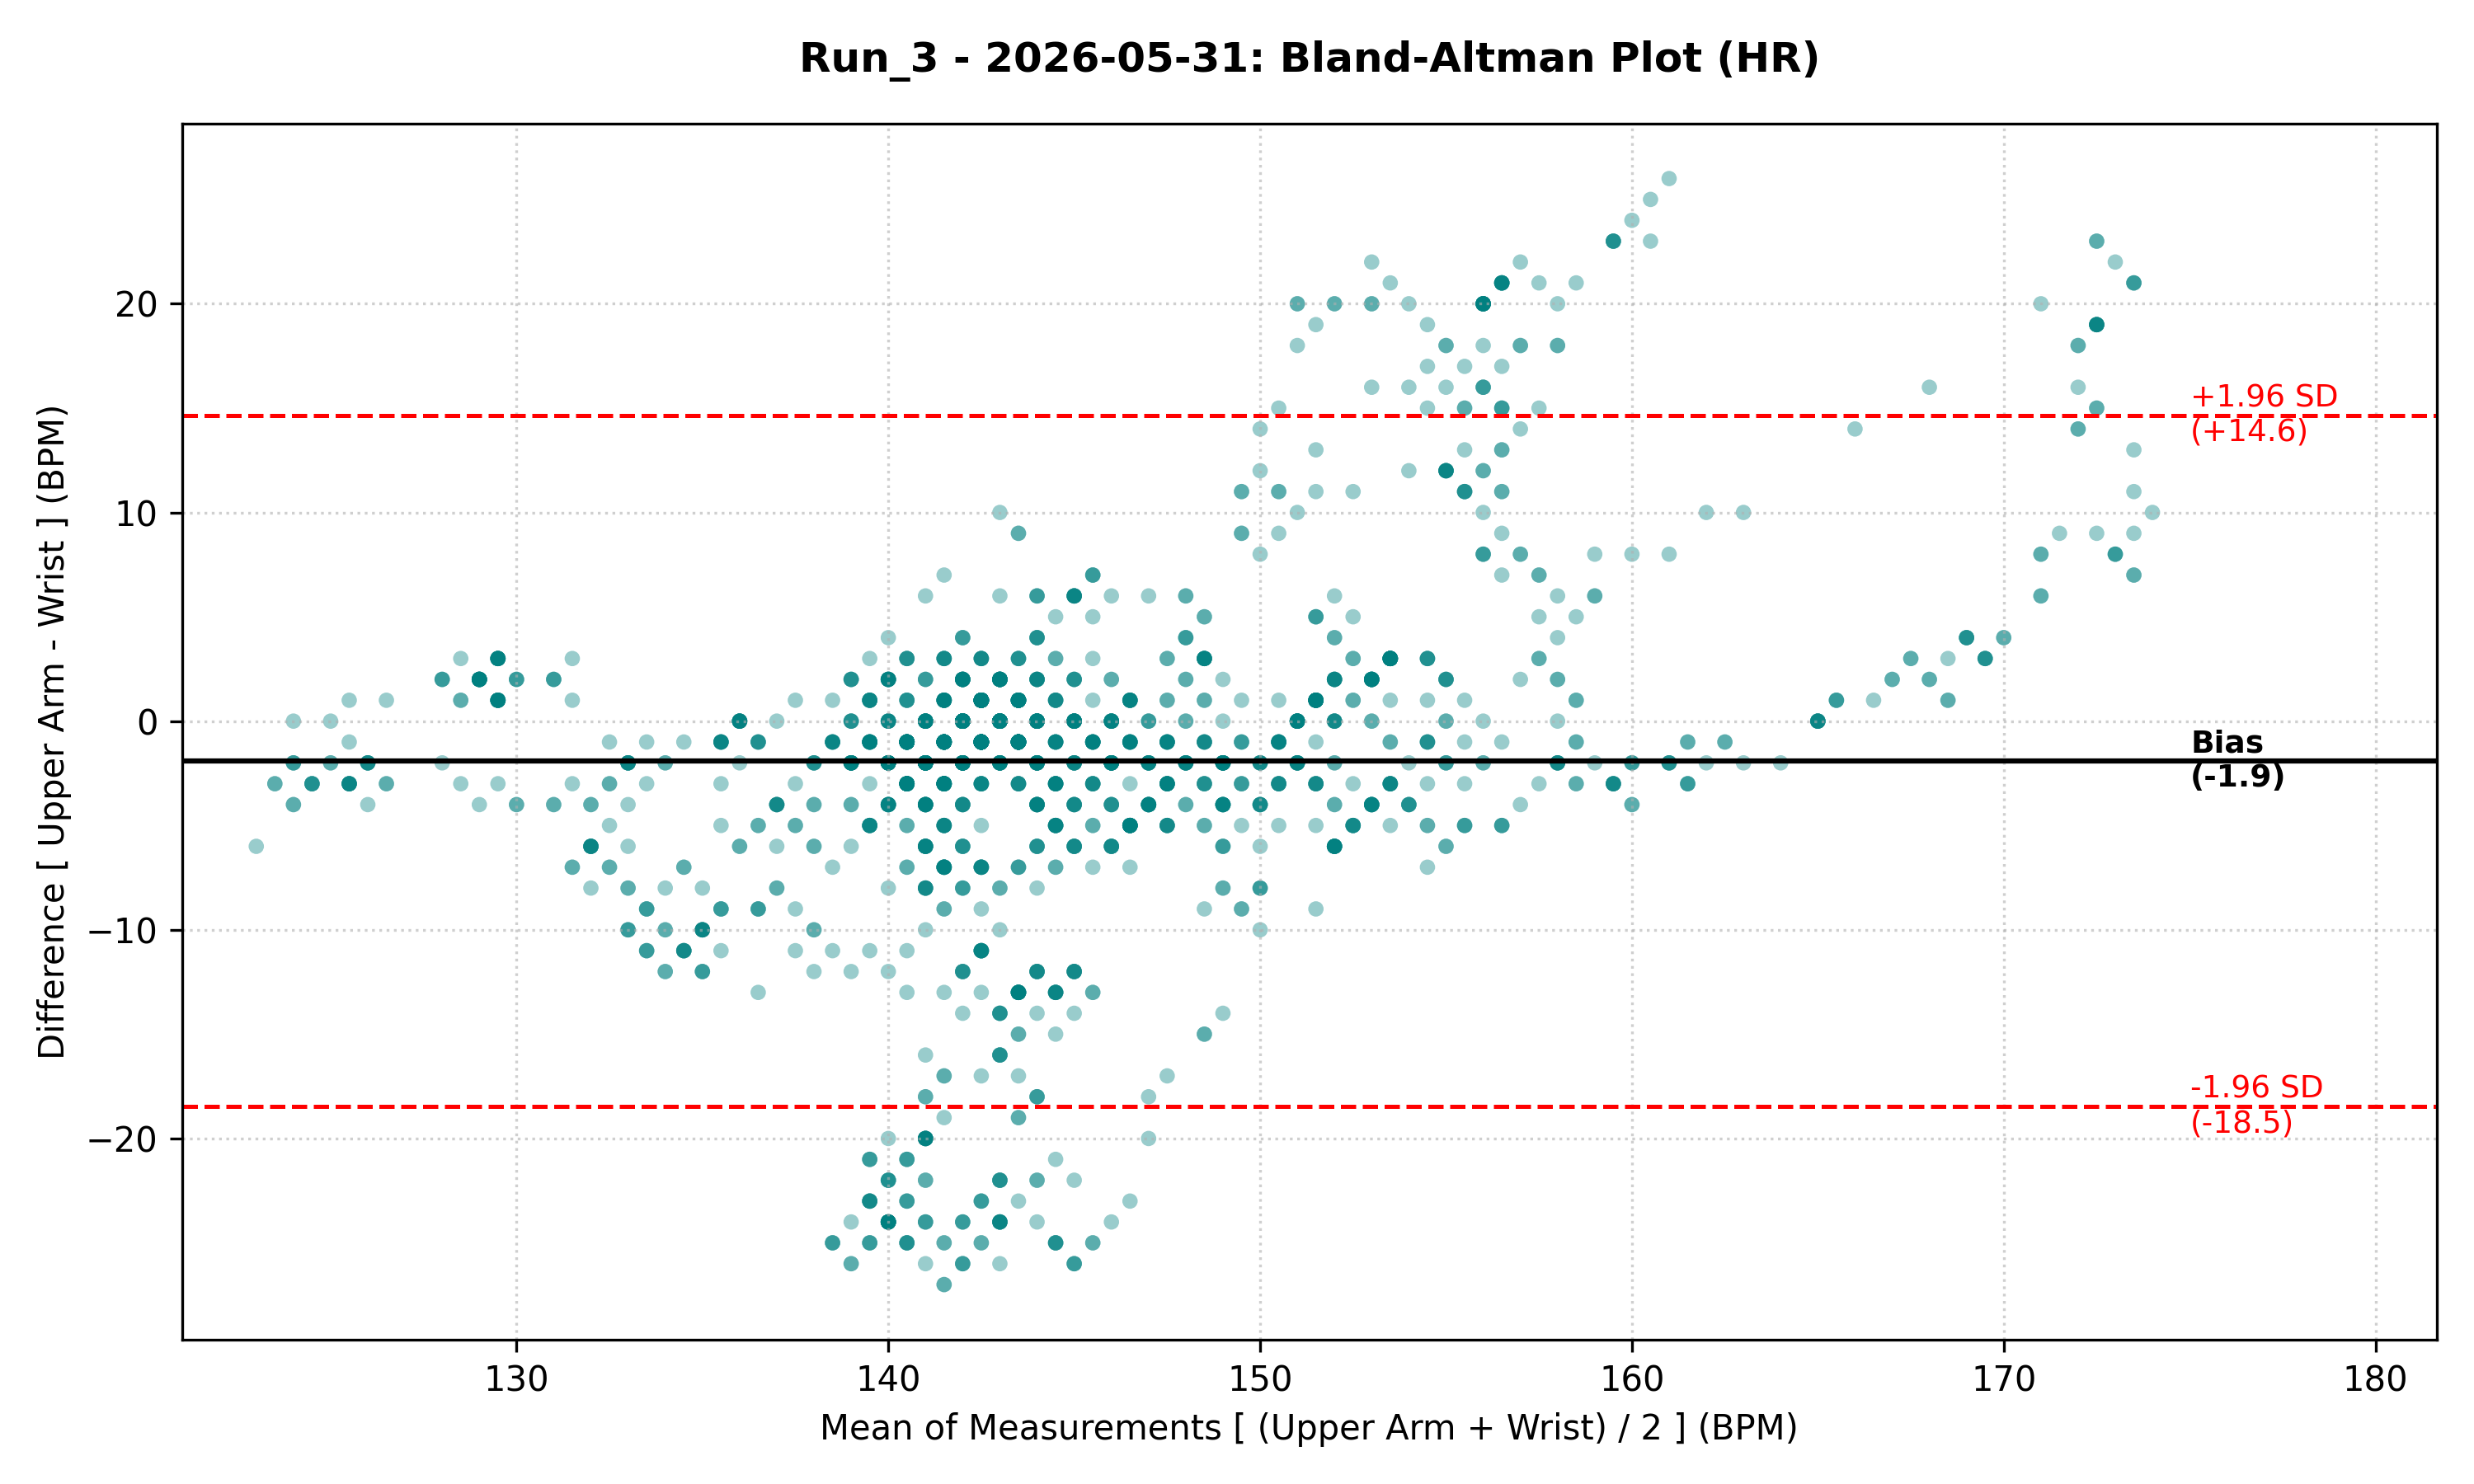
\includegraphics[width=\linewidth]{Run_3_HR_Bland_Altman.png}
			\caption{Bland-Altman plot (Trial 3, Bias $=-1.9$\,bpm)}
		\end{subfigure}
		\caption{Statistical agreement between upper-arm and wrist sensors for
			Trial 3. The scatterplot (a) reveals a moderate correlation with
			notable spread. The Bland-Altman plot (b) shows a small mean bias
			($-1.9$\,bpm) but wide 95\% limits of agreement ($+14.6$ to
			$-18.5$\,bpm), with underestimation by the wrist sensor increasingly
			visible at higher heart rates. Trial~3 is close to the cross-run
			\emph{median} agreement (Figure~\ref{fig:hragreement}), but not to the
			cross-run \emph{mean}, which is pulled down by Run~2.}
		\label{fig:agreement}
	\end{figure}
	
	\begin{figure}[!htb]
		\centering
		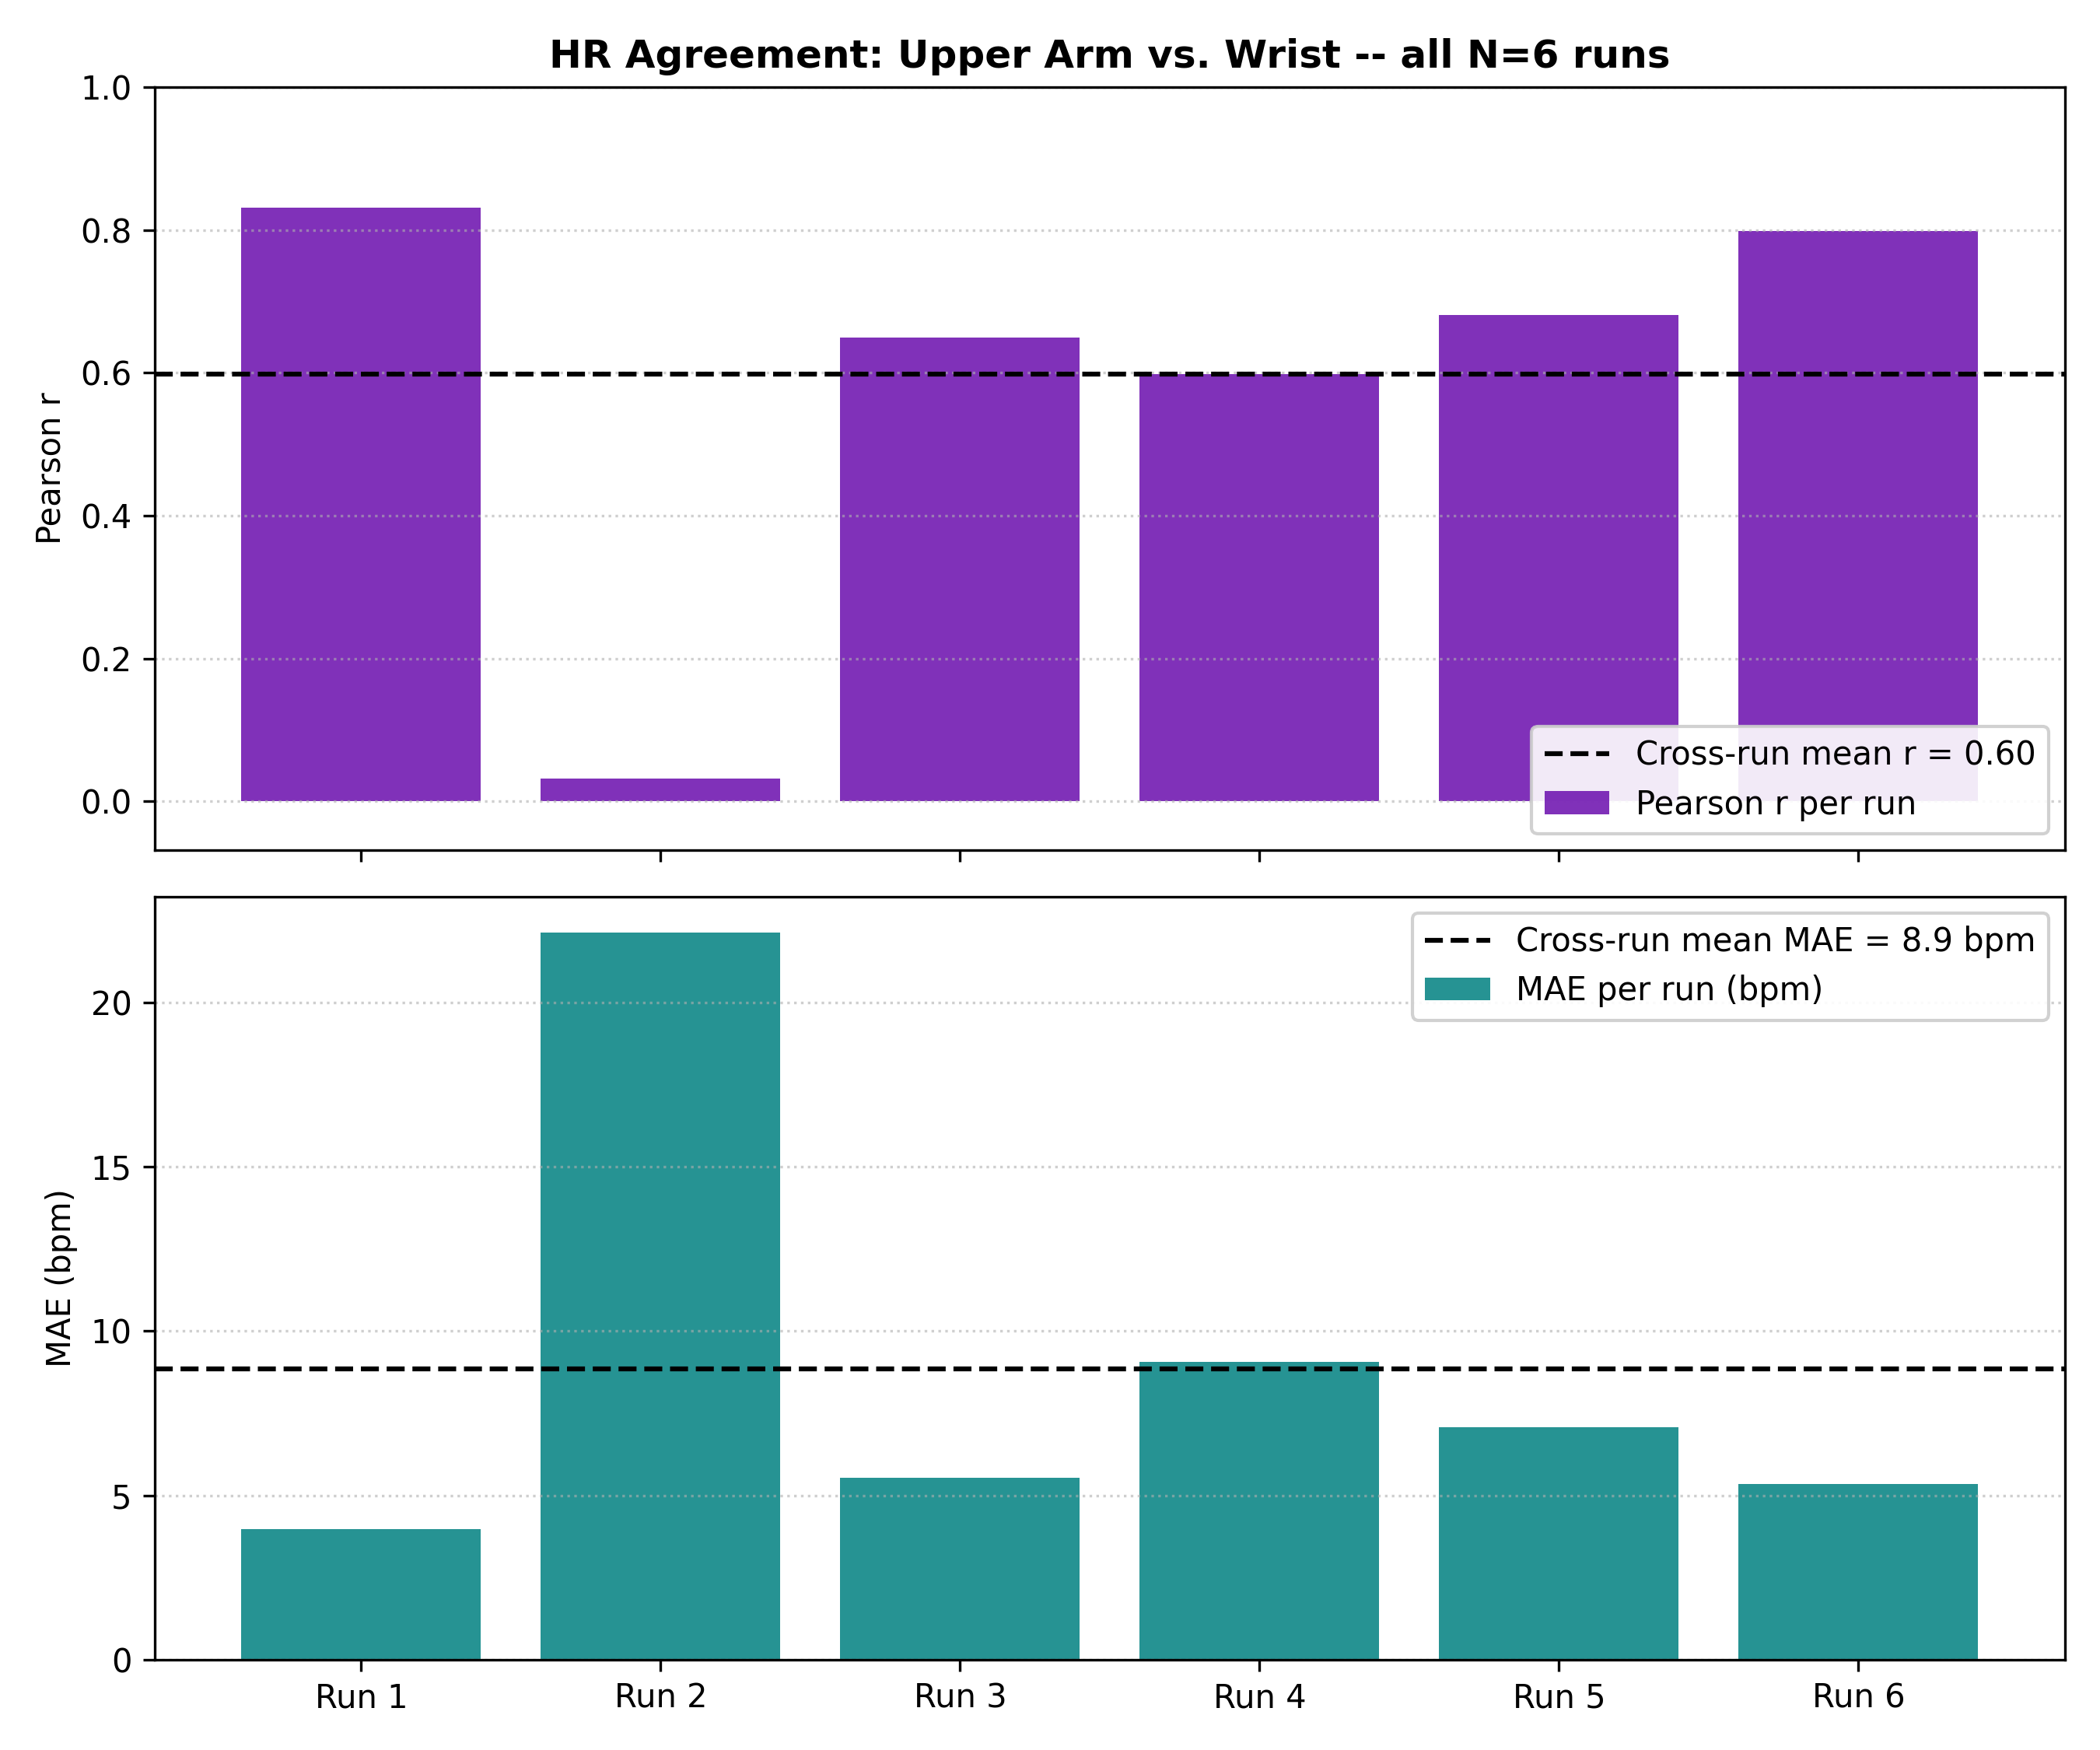
\includegraphics[width=\linewidth]{hr_agreement_all_runs.png}
		\caption{HR agreement (Pearson $r$, top; MAE, bottom) between
			upper-arm and wrist sensors across all $N=6$ runs. Cross-run mean
			$r=0.60$ (median $0.66$) and mean MAE $=8.9$\,bpm. The single-trial
			example in Figure~\ref{fig:agreement} ($r=0.65$) closely matches the
			cross-run \emph{median}, but the \emph{mean} is pulled substantially
			lower by Run~2 ($r=0.03$, MAE $=22.1$\,bpm), illustrating why a single
			representative trial can understate the overall variance in device
			agreement (see Section~5).}
		\label{fig:hragreement}
	\end{figure}
	
	Figure~\ref{fig:blandaltmangrid} shows the individual Bland-Altman plots
	underlying this aggregate view, most clearly visualizing the Run~2
	anomaly discussed in Section~5.
	
	\begin{figure*}[!htb]
		\centering
		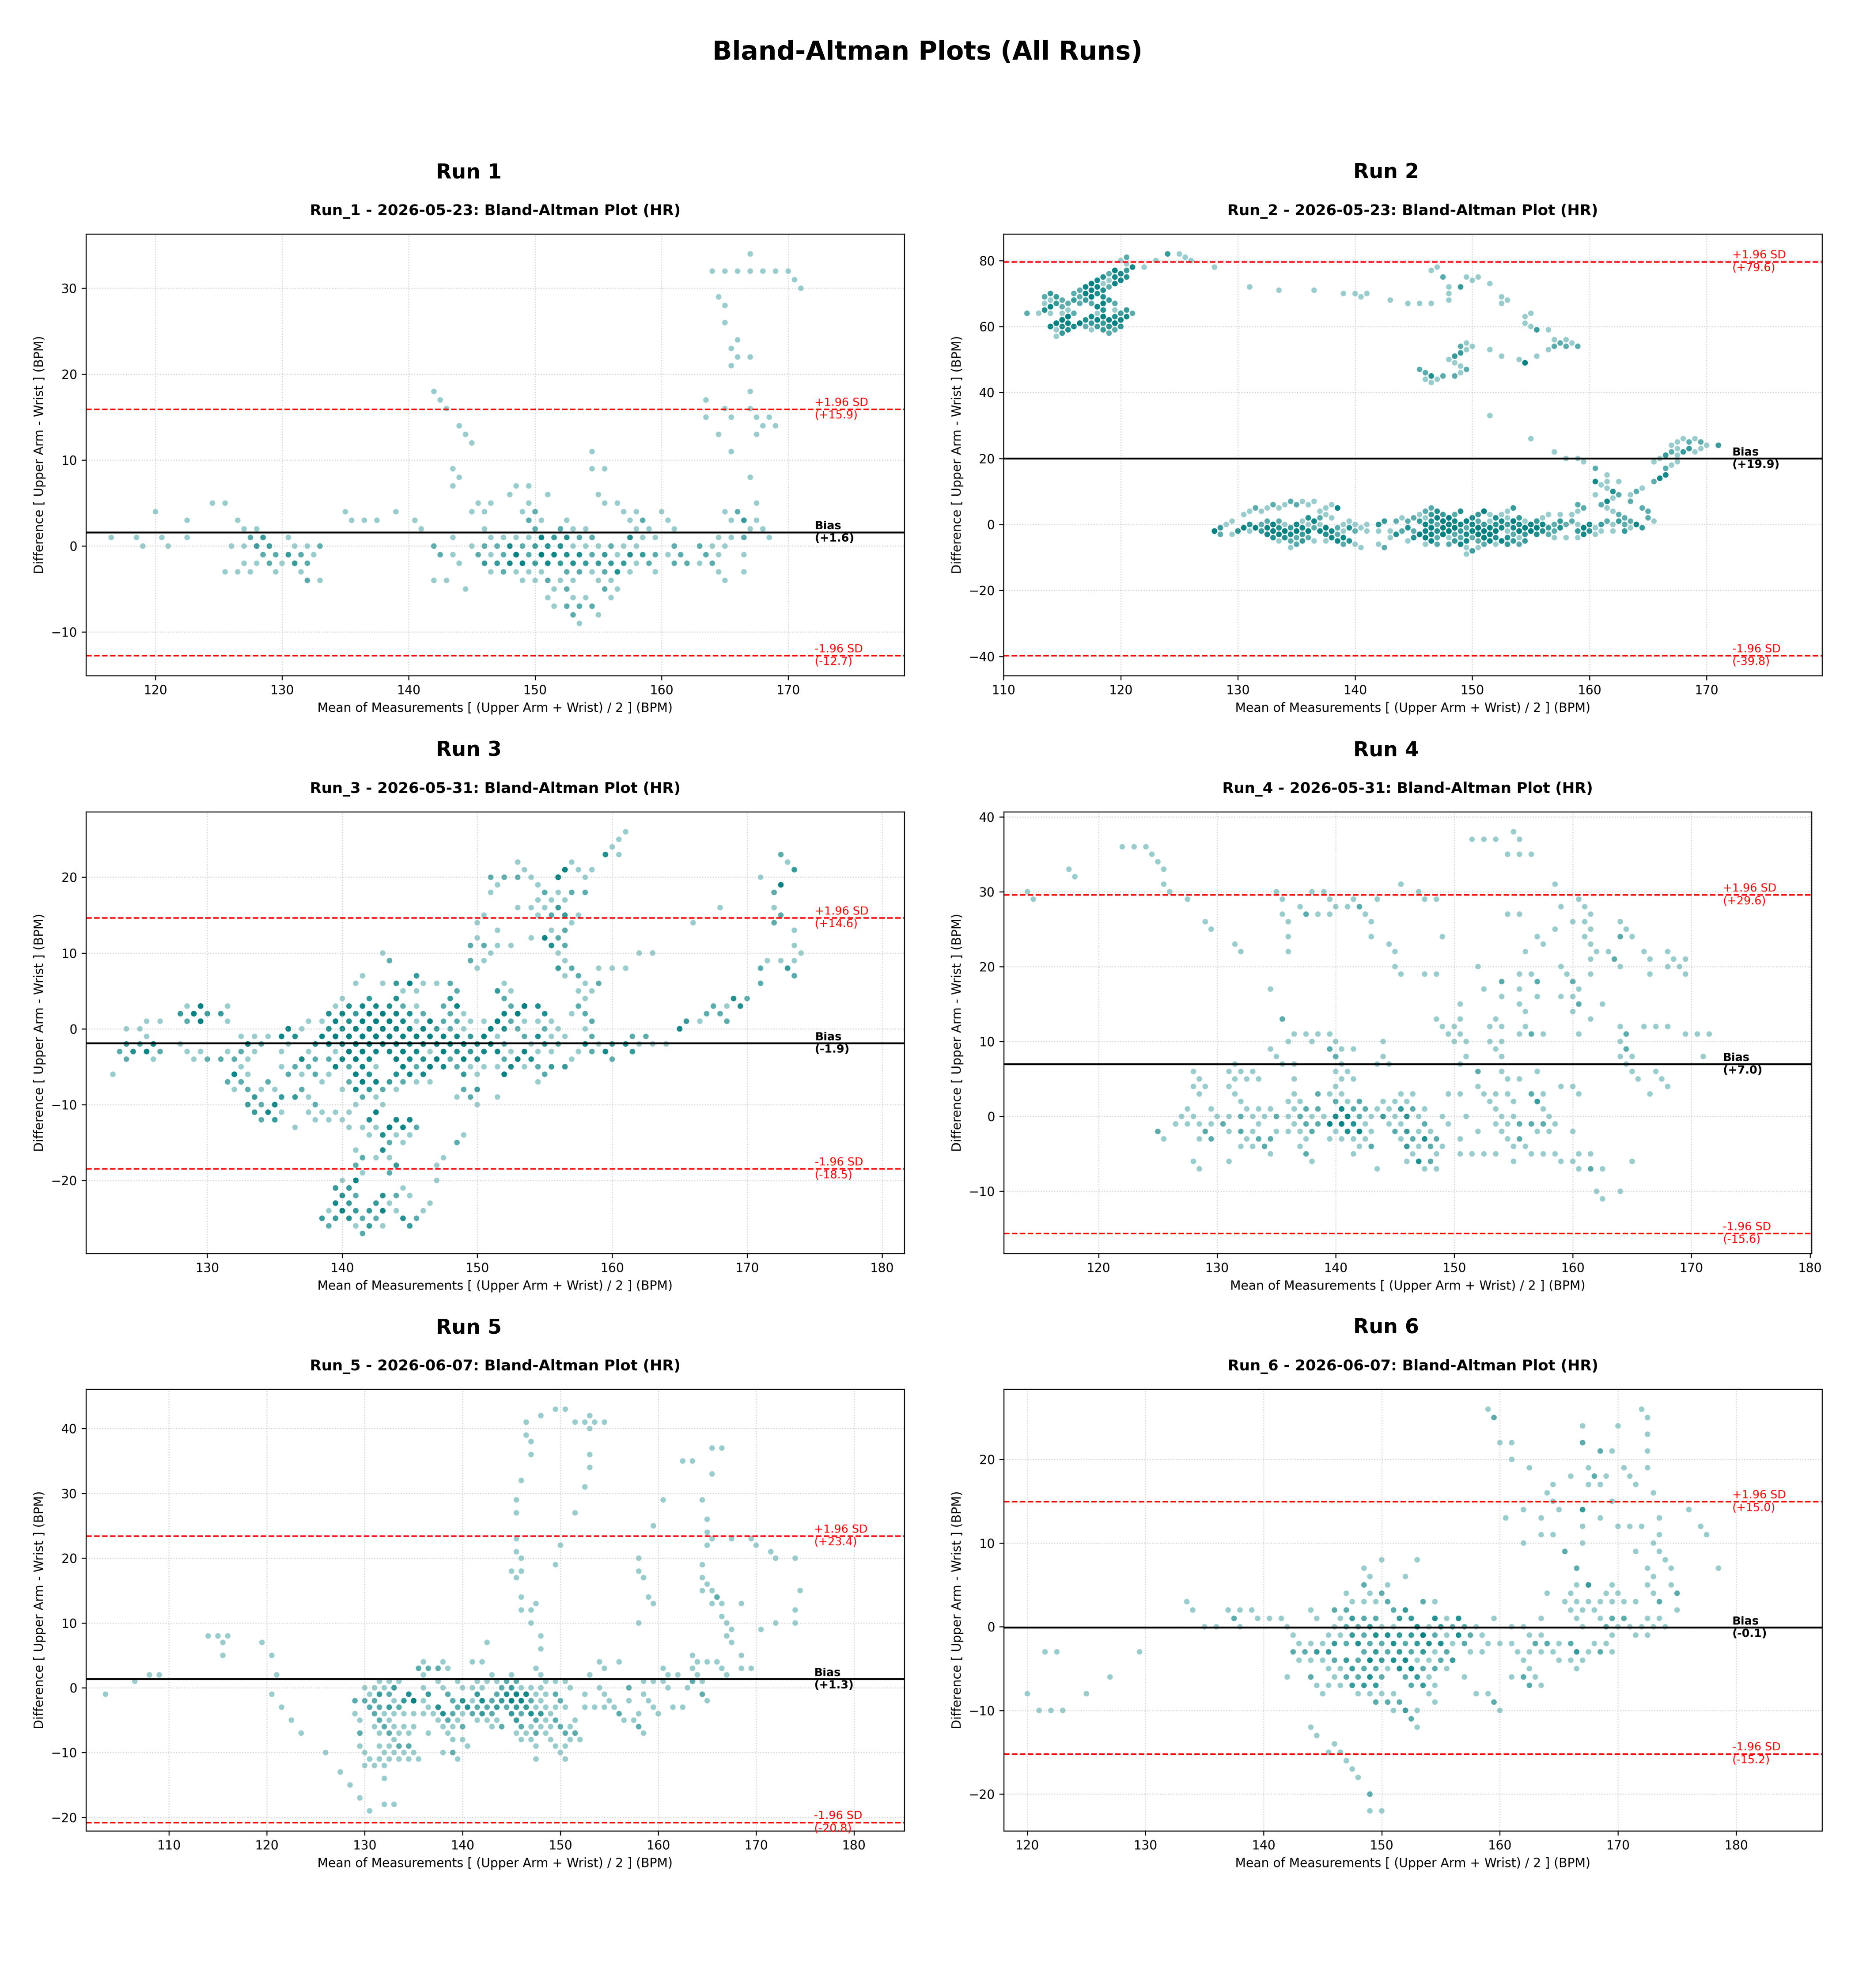
\includegraphics[width=0.85\linewidth]{Bland_Altman_Grid_3x2.png}
		\caption{Bland-Altman plots for all $N=6$ runs individually. Run~1,
			3, 5, and 6 show the expected pattern of tight agreement with modest
			bias; Run~4 shows a persistent positive bias; Run~2 shows the
			characteristic three-cluster split described in Section~5, a direct
			visual signature of the cadence-lock event rather than random
			measurement noise.}
		\label{fig:blandaltmangrid}
	\end{figure*}
	
	\begin{figure}[!htb]
		\centering
		\begin{subfigure}[b]{0.9\linewidth}
			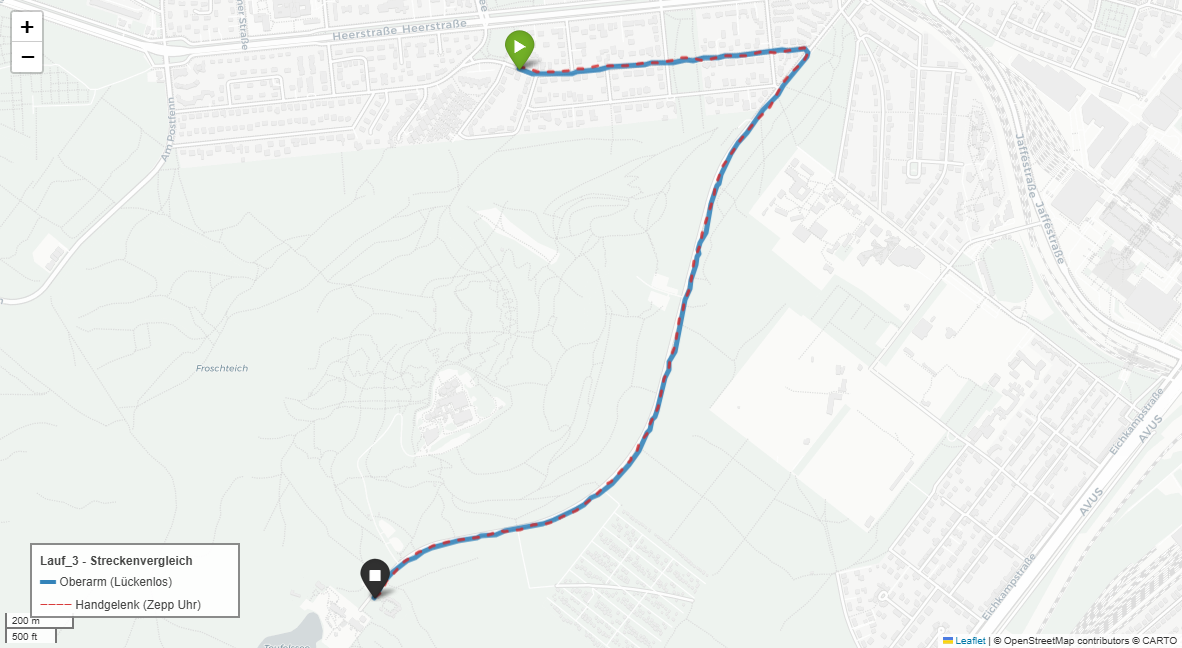
\includegraphics[width=\linewidth]{run_3_route.png}
			\caption{Route comparison, Trial 3 (mean offset 8.26\,m, max.\ 22.9\,m for this run)}
		\end{subfigure}\par\vspace{2mm}
		\begin{subfigure}[b]{0.9\linewidth}
			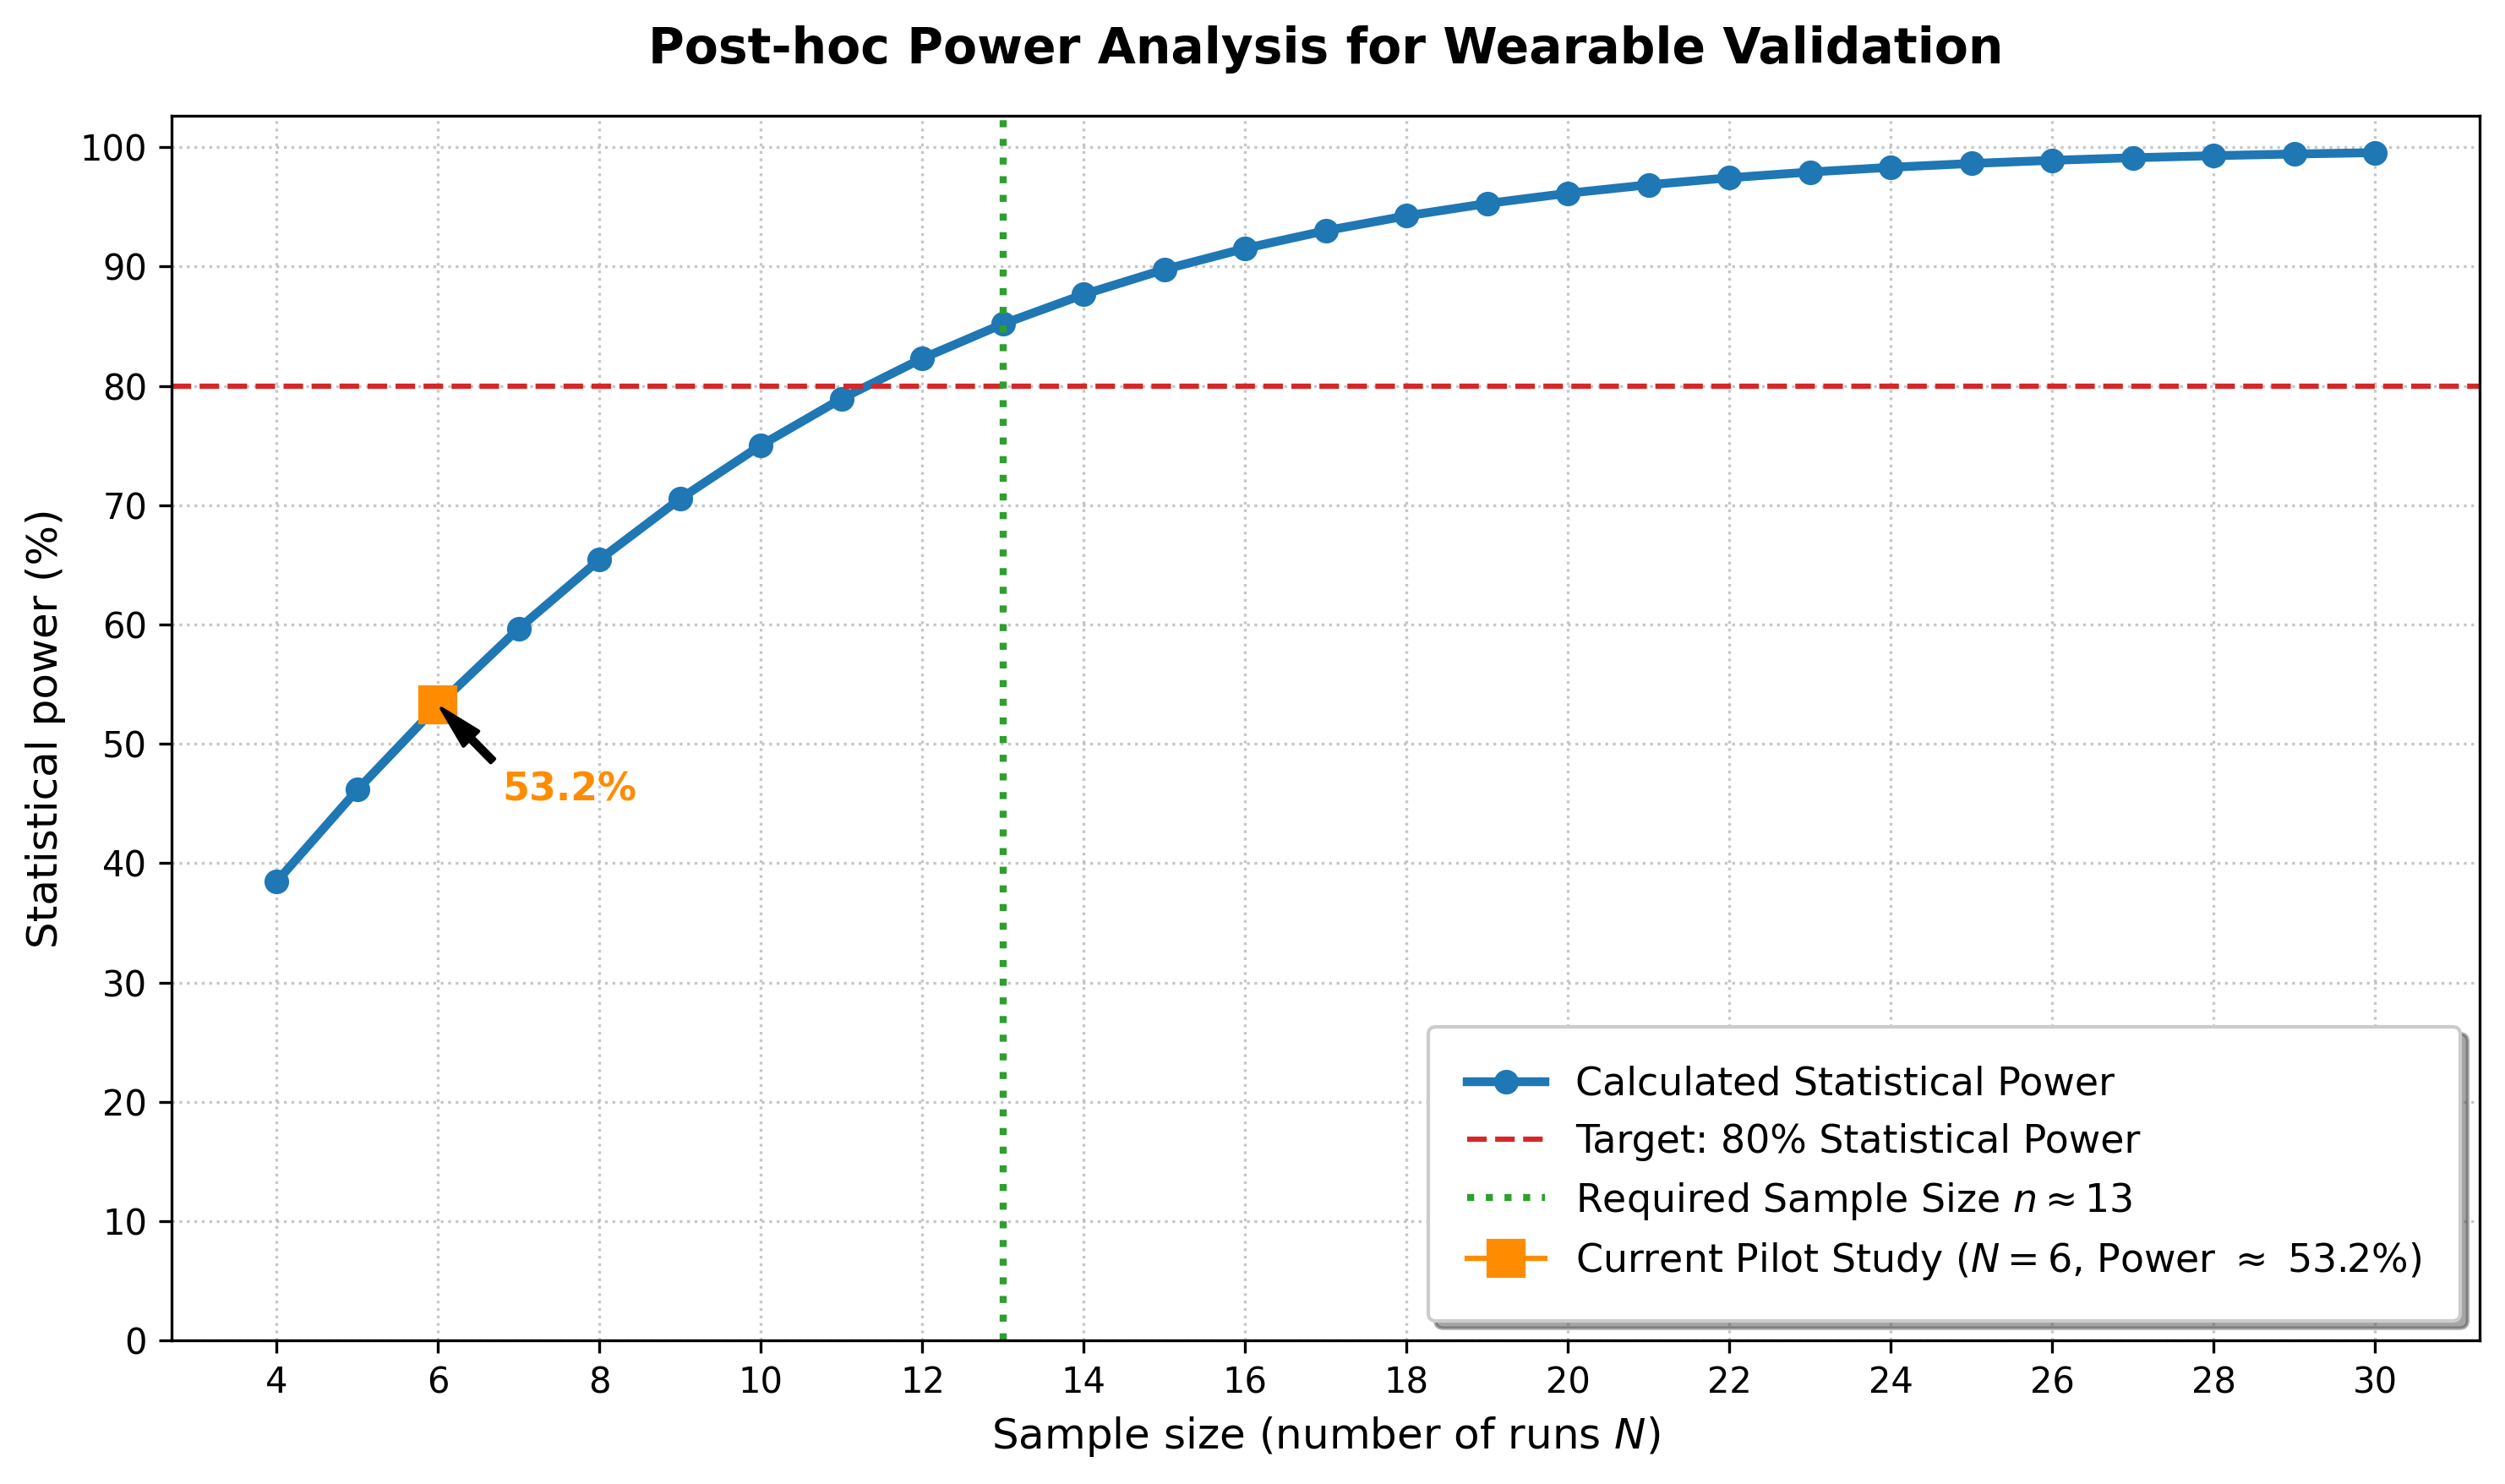
\includegraphics[width=\linewidth]{power_analysis_curve.png}
			\caption{Post-hoc power analysis ($\Delta=5$\,bpm, $\sigma_d=6$\,bpm, $\alpha=0.05$)}
		\end{subfigure}
		\caption{Geospatial tracking accuracy for Trial 3 (a) and statistical
			power validation (b). $N=6$ achieves 53.2\% power; $n\approx13$ trials
			would be required for the conventional 80\% target.}
		\label{fig:power}
	\end{figure}
	
	\begin{figure}[!htb]
		\centering
		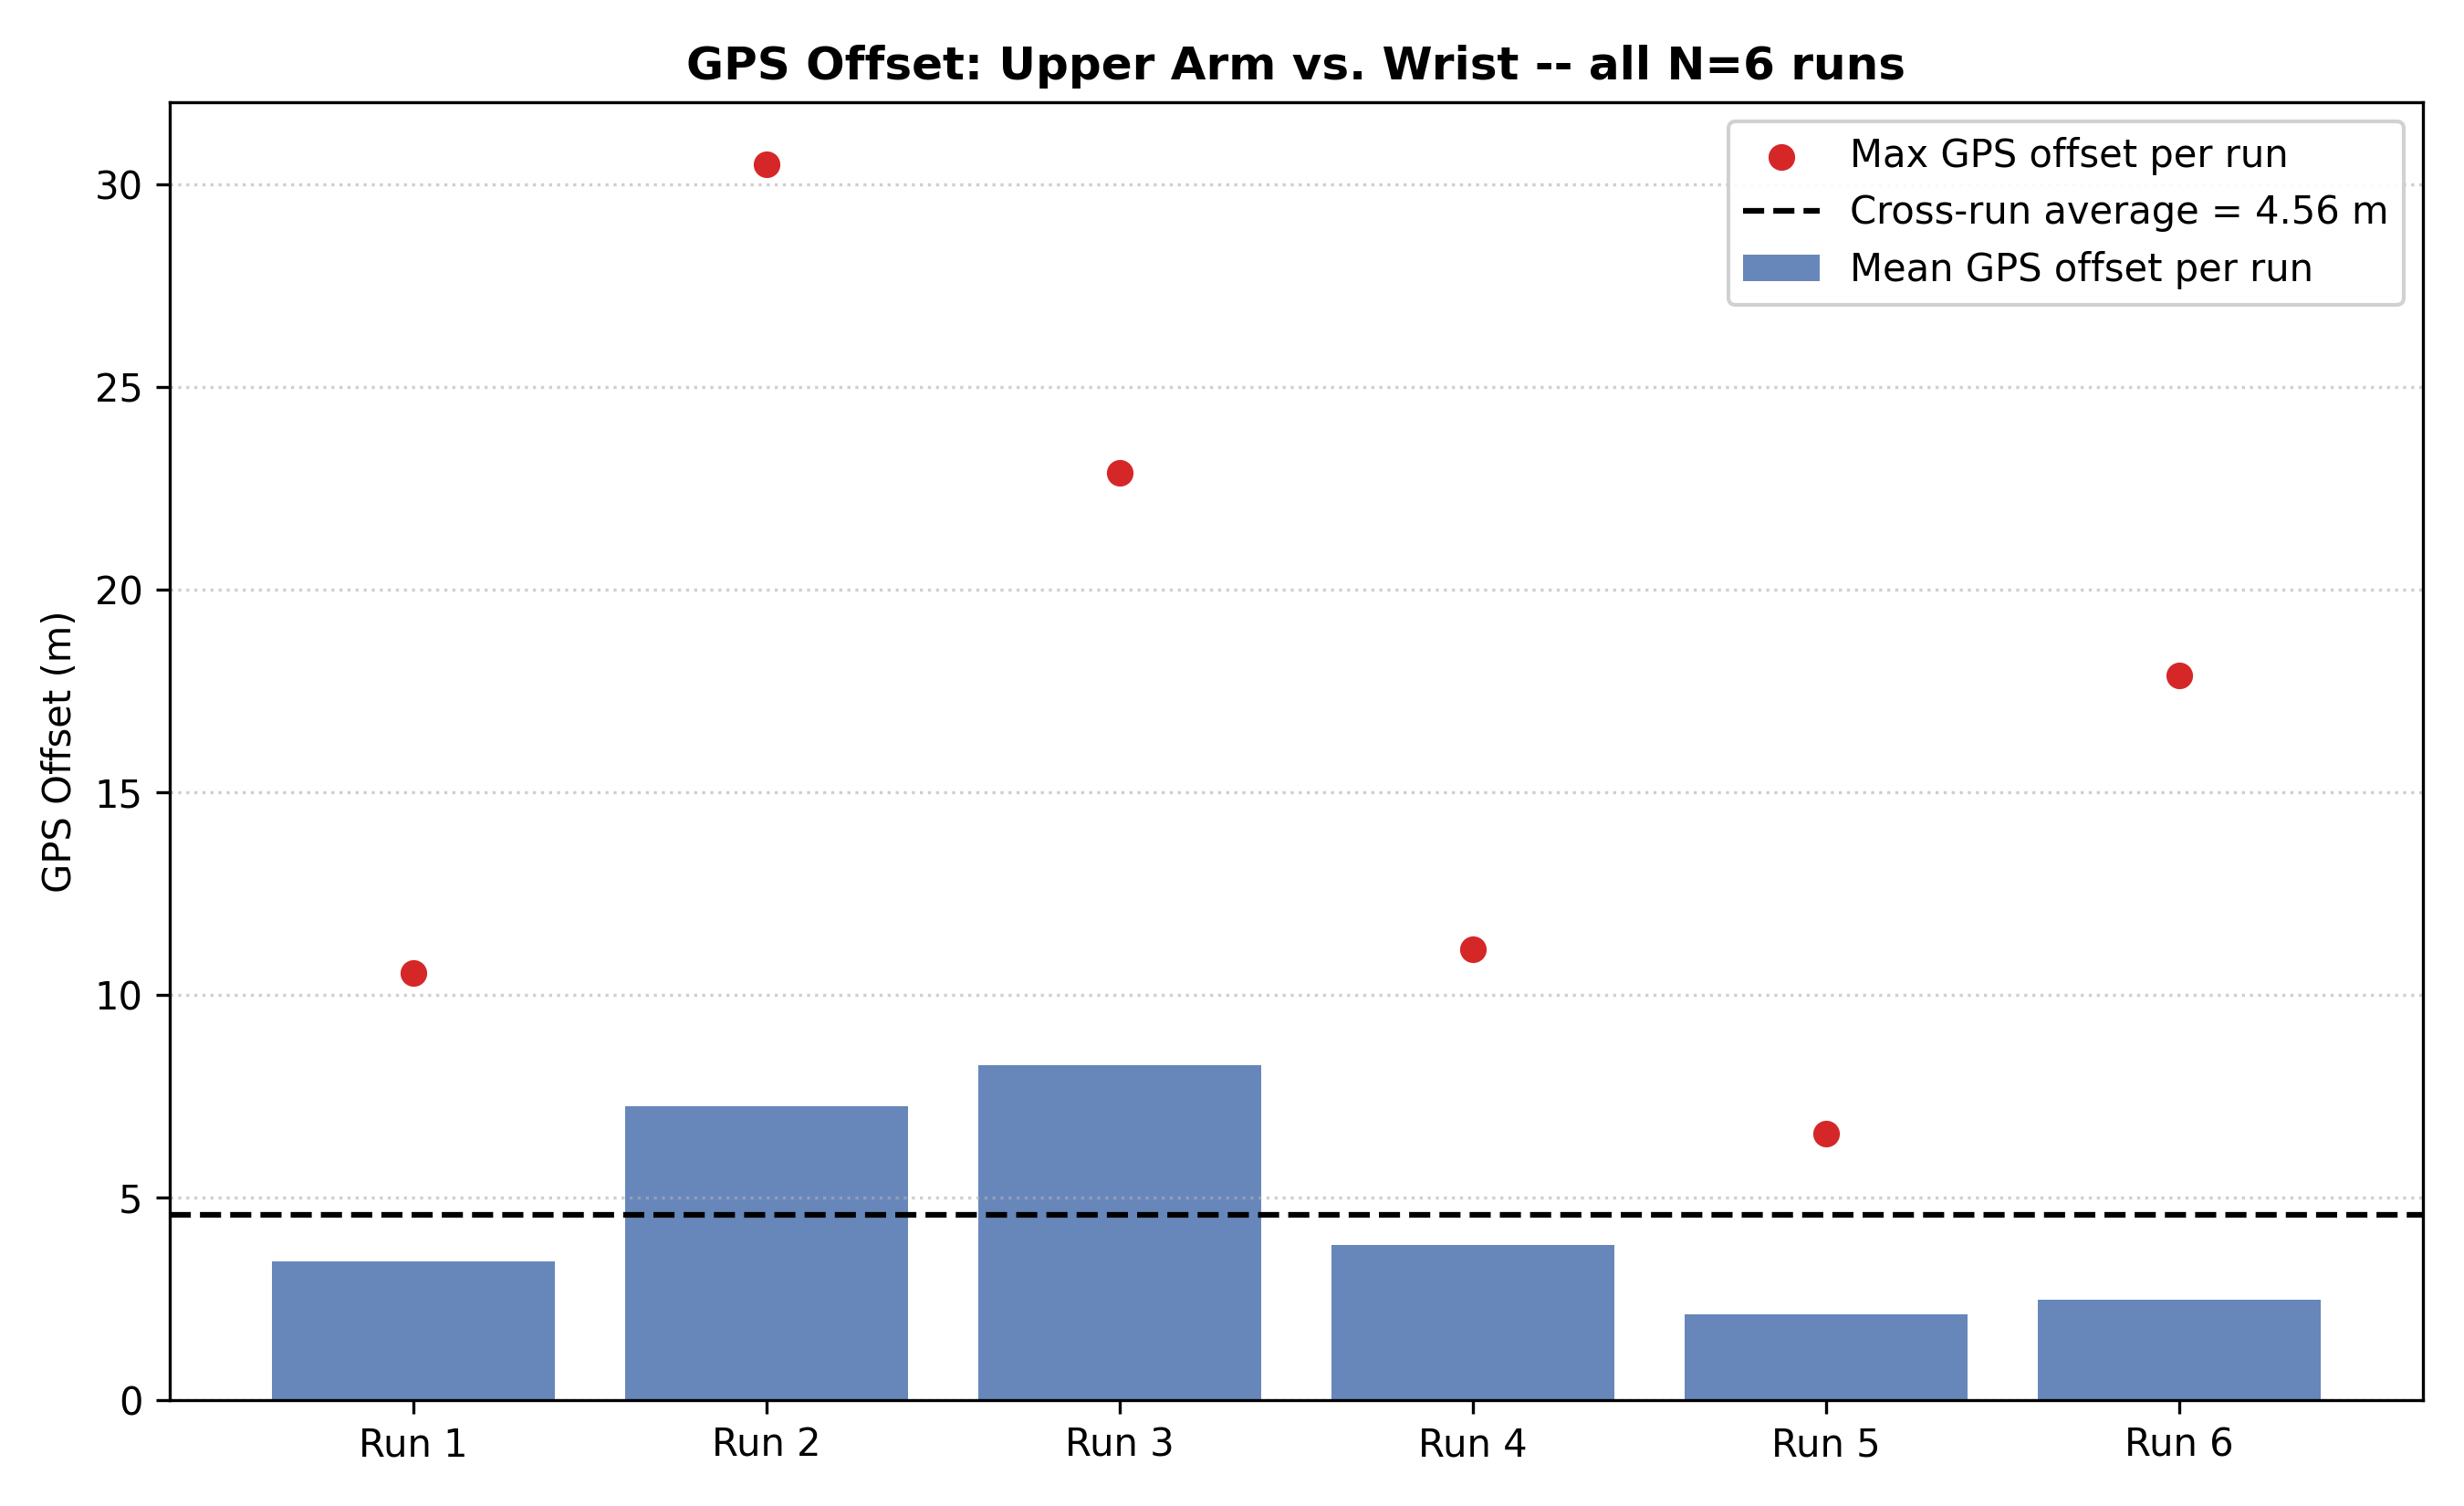
\includegraphics[width=\linewidth]{gps_offset_all_runs.png}
		\caption{GPS offset between upper-arm and wrist tracks across all
			$N=6$ runs. The cross-run mean (4.56\,m, dashed line) is the
			representative figure reported in the Abstract; per-run means range
			from 2.1 to 8.3\,m, with individual maxima up to 30.5\,m (Run 2).}
		\label{fig:gpsoffset}
	\end{figure}
	
	\begin{figure}[!htb]
		\centering
		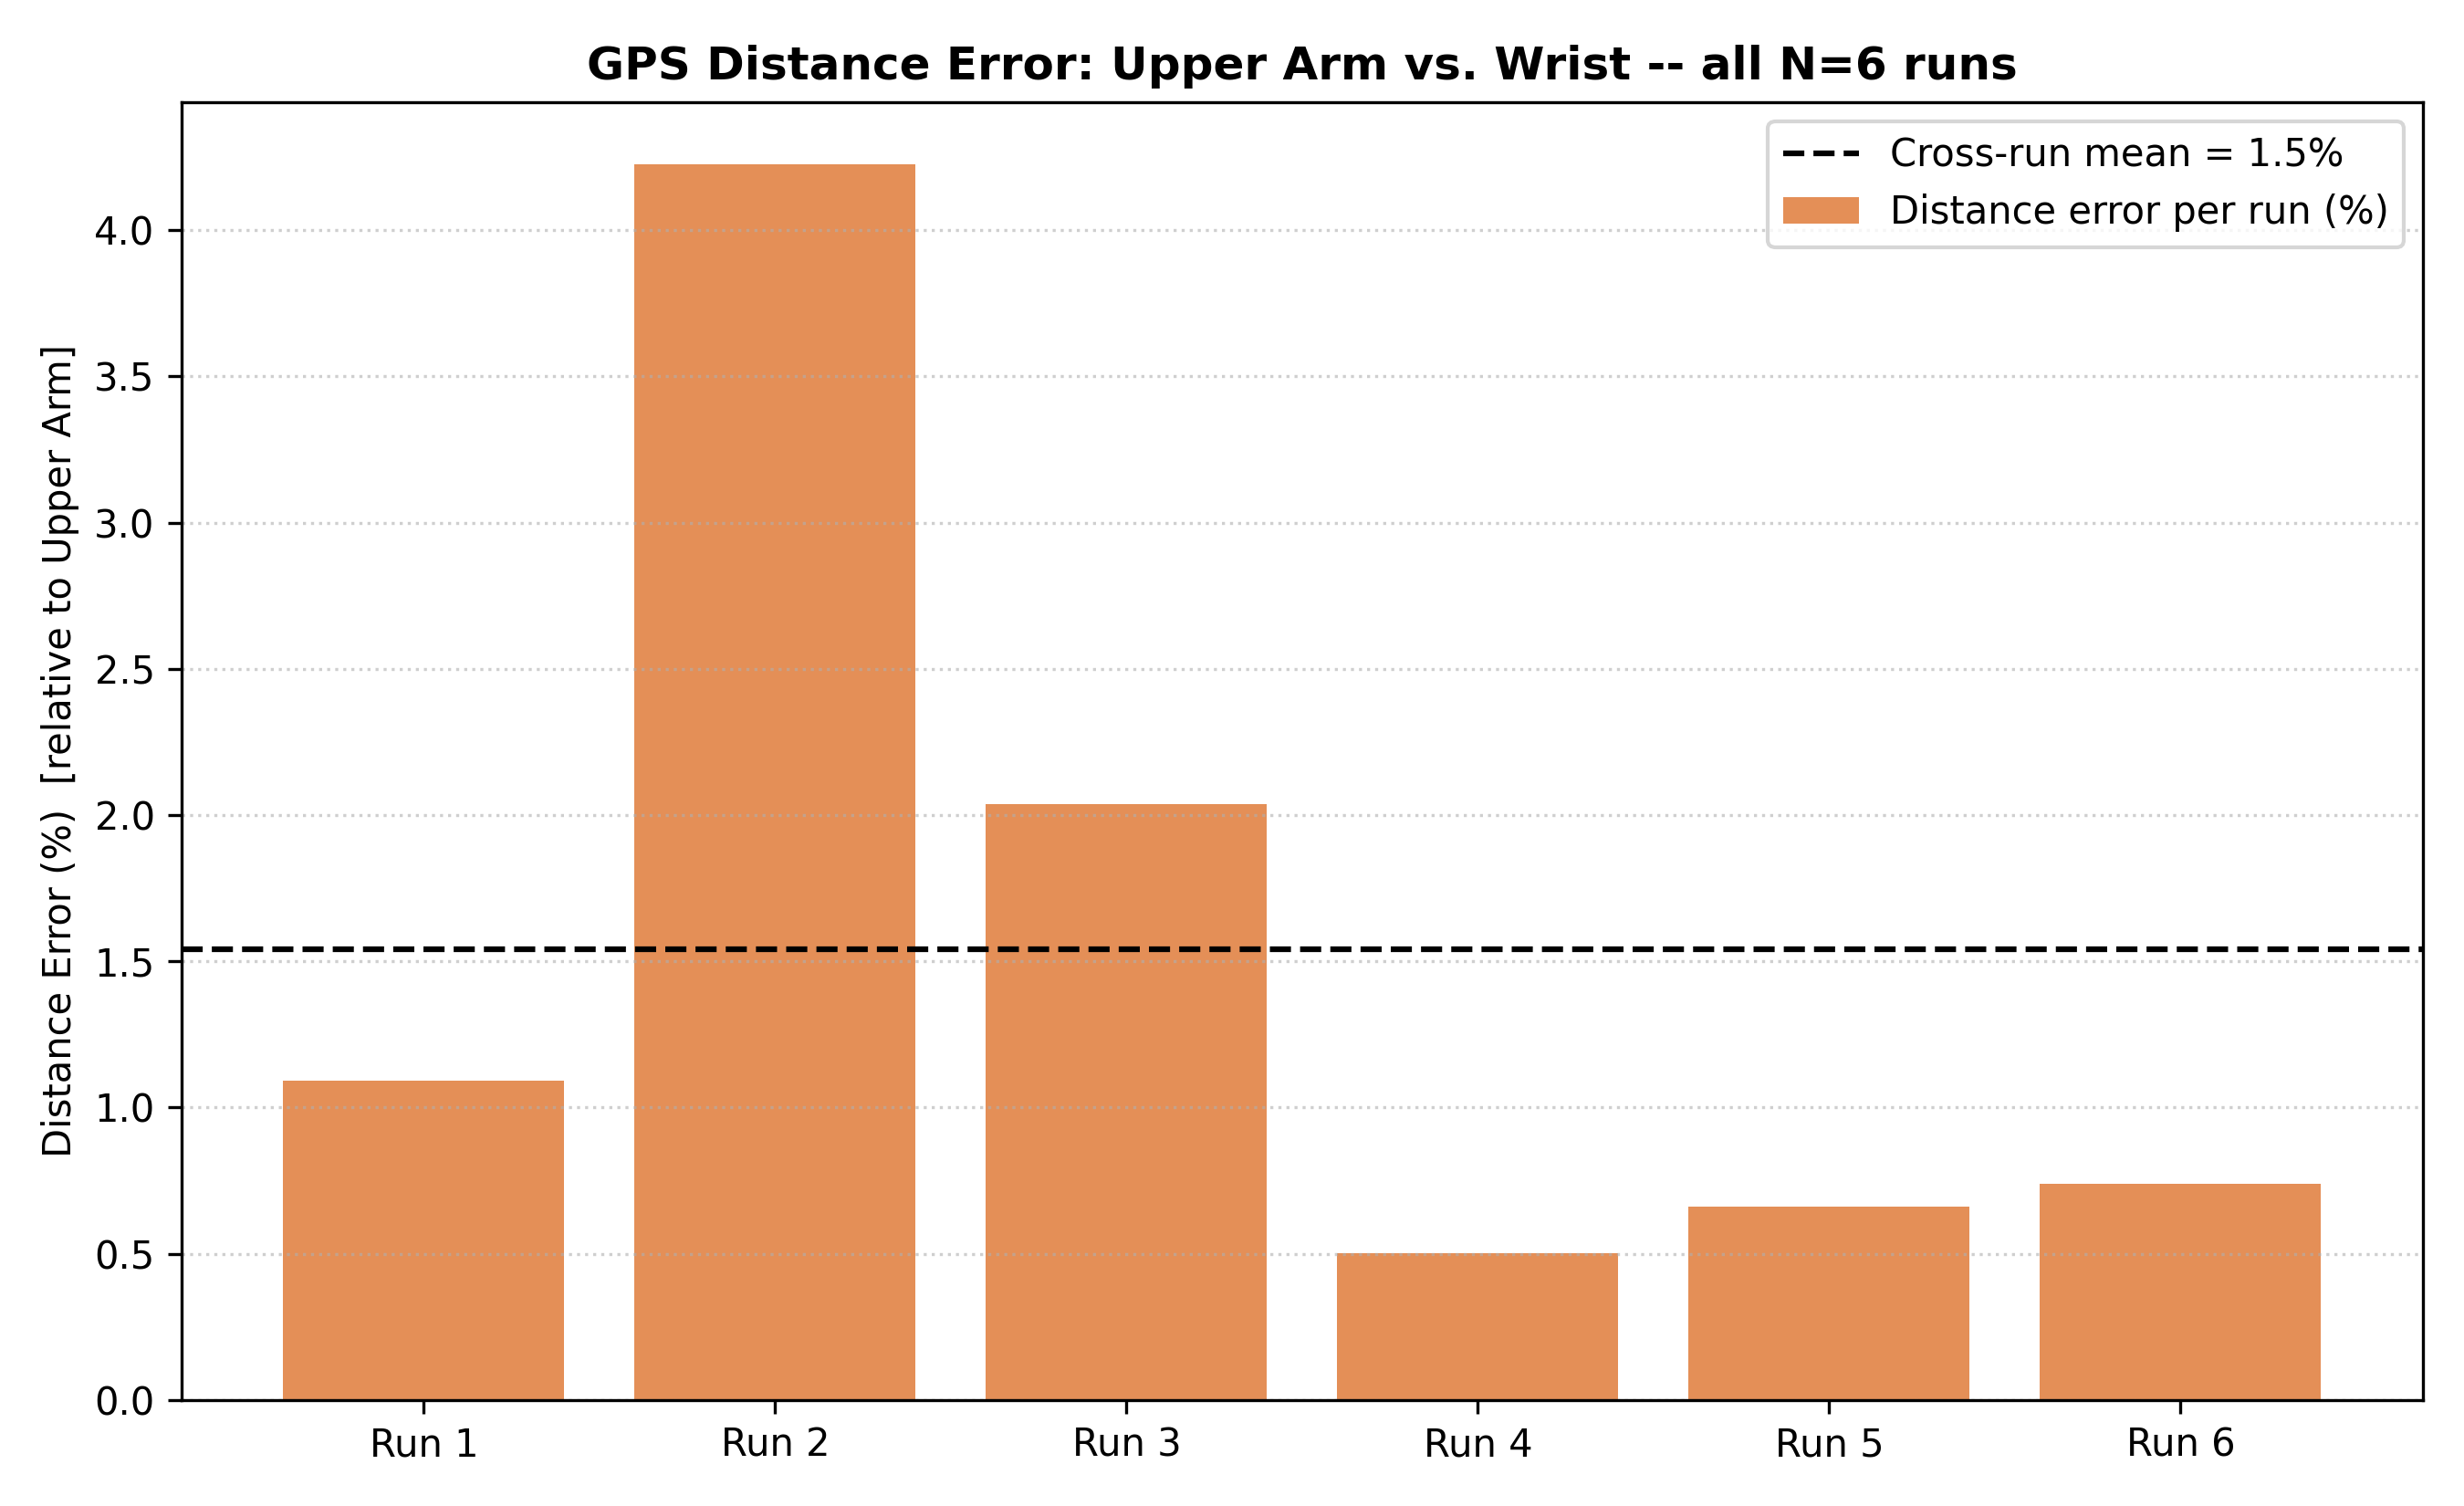
\includegraphics[width=\linewidth]{distance_error_all_runs.png}
		\caption{Relative GPS track-length error (upper arm as reference)
			across all $N=6$ runs. The cross-run mean (1.5\%, dashed line) is
			again driven up by Run~2 (4.2\%), consistent with the GPS-offset and
			HR-agreement outliers observed for the same run (see Section~5).}
		\label{fig:distanceerror}
	\end{figure}
	
	\subsection{Sample Size \& Power Validation}
	
	In contemporary hardware validation literature for optical heart rate
	sensors, sample sizes typically range from 30 to 50 \emph{participants}
	\cite{jacko_validity_2024,chow_accuracy_2020,stahl_how_2016} --- a figure not directly comparable
	to our $n\approx13$ \emph{trials}, since our design uses repeated trials
	from a single subject rather than multiple participants (see
	Section~5). To determine the statistical scalability of our $N=6$
	longitudinal trial matrix, a post-hoc power analysis was conducted for a
	two-sided paired $t$-test using Equation~\ref{eq:power}:
	
	\begin{equation}
		n = \frac{(Z_{1-\alpha/2}+Z_{1-\beta})^2 \cdot \sigma_d^2}{\Delta^2}
		\label{eq:power}
	\end{equation}
	
	Where $\alpha=0.05$ ($Z_{0.975}=1.96$), $1-\beta=0.80$ ($Z_{0.80}=0.84$),
	$\Delta=5$\,bpm specifies the targeted minimal detectable difference, and
	$\sigma_d=6$\,bpm is the standard deviation of differences.
	
	As illustrated in Figure~\ref{fig:power}(b), solving Equation~\ref{eq:power}
	yields a required sample size of $n\approx13$ to achieve 80\% statistical
	power. The current sample size of $N=6$ reaches approximately 53.2\% of
	that target. This study should therefore be read as an
	\textbf{underpowered, exploratory pilot}: it is useful for identifying
	structural sensor differences worth investigating further, but it is not
	a confirmatory validation, and effect sizes reported here should not be
	generalized without a larger, adequately powered, multi-subject
	replication.
	
	% ---------------------------------------------------------------
	\section{Discussion \& Limitations}
	
	The primary structural vulnerability of the wrist-worn architecture
	appears to be motion artifacts rather than the optical algorithm itself.
	Rapid arm accelerations shift the watch body, causing ambient light
	leakage. This is consistent with the observation that the wrist device's
	companion app omitted over 1,000 seconds of data in multiple runs, a
	vulnerability similarly reported for other wrist-worn PPG technologies
	subjected to arm movement \cite{schweizer2024heart}. In Run~2, a
	\emph{cadence lock} occurred: the wrist strap loosened, causing the
	device to lock onto the stride rhythm ($\sim$130\,bpm) instead of the
	cardiovascular load ($\sim$150\,bpm).
	
	Notably, this single event coincides with Run~2 being an outlier across
	\emph{several} independently measured dimensions: HR agreement collapses
	($r=0.03$, MAE $=22.1$\,bpm, bias $=+19.9$\,bpm), GPS offset peaks
	(30.5\,m, more than $6\times$ the cross-run mean), track-length error is
	highest (4.2\%, roughly $3\times$ the cross-run mean of 1.5\%;
	Figure~\ref{fig:distanceerror}), and the
	estimated HR time lag (+60\,s) sits exactly at the boundary of the
	$\pm60$\,s search window used for the cross-correlation, meaning the true
	lag may exceed the tested range and the reported value should be treated
	as a lower bound rather than a precise estimate. The convergence of
	degraded agreement, offset, and lag metrics in a single run --- rather
	than four independent anomalies scattered across different trials ---
	supports the interpretation that a single mechanical event (the loosened
	strap) is the common cause, and cautions against averaging Run~2 together
	with the other five runs without flagging it as qualitatively different.
	
	Speed agreement, however, does \emph{not} follow this pattern: Run~2
	achieves $r=0.72$, close to the cross-run mean ($r=0.73$), while Run~1
	--- otherwise the cleanest run for HR agreement ($r=0.83$) --- shows the
	\emph{weakest} speed agreement of all six runs ($r=0.55$). This
	dissociation is informative rather than contradictory: PPG-derived HR and
	GPS-derived position are both sensitive to strap tightness and skin
	contact, whereas the wrist device's speed estimate can draw on
	accelerometer/gyroscope data largely independent of optical or GPS
	quality, plausibly explaining why it degrades on a different run and by
	a different mechanism. Consequently, the ``single confound'' account
	below should be read as applying specifically to the optical and GPS
	subsystems, not to the device as a whole.
	
	This convergence is not merely visual: treating each run's summary
	statistic as one observation ($N=6$), several of these degradation
	metrics correlate significantly with each other across runs
	(Table~\ref{tab:correlations}). Distance error correlates strongly with
	both weaker HR agreement ($r=-0.89$, $p=0.018$) and higher HR MAE
	($r=+0.84$, $p=0.035$), and HR lag correlates with weaker HR agreement
	($r=-0.84$, $p=0.038$). Speed agreement, by contrast, shows essentially
	no correlation with any of these metrics ($|r|<0.25$ in all cases),
	consistent with the dissociation noted above. Given $N=6$ these
	correlations should be read as suggestive rather than confirmatory, but
	they are consistent with a single latent factor --- optical/GPS
	attachment quality in a given run --- driving degradation jointly across
	the HR and geospatial channels, while speed tracking degrades through a
	separate, uncorrelated mechanism.
	
	\begin{table}[!htb]
		\centering
		\caption{Cross-run correlations ($N=6$ runs treated as observations)
			between degradation metrics. Distance error and HR lag both correlate
			significantly with weaker HR agreement, supporting a shared underlying
			cause; speed agreement correlates with none of them, suggesting it fails
			independently.}
		\label{tab:correlations}
		\small
		\begin{tabular}{lcc}
			\toprule
			Metric pair & Pearson $r$ & $p$ \\
			\midrule
			Distance error vs.\ HR $r$   & $-0.89$ & $0.018$ \\
			Distance error vs.\ HR MAE   & $+0.84$ & $0.035$ \\
			HR lag vs.\ HR $r$           & $-0.84$ & $0.038$ \\
			GPS mean offset vs.\ distance error & $+0.77$ & $0.075$ \\
			GPS max offset vs.\ HR $r$   & $-0.73$ & $0.100$ \\
			GPS mean offset vs.\ HR $r$  & $-0.59$ & $0.215$ \\
			\midrule
			Speed $r$ vs.\ HR $r$        & $-0.18$ & $0.727$ \\
			Speed $r$ vs.\ distance error & $-0.11$ & $0.840$ \\
			Speed $r$ vs.\ GPS max offset & $-0.05$ & $0.922$ \\
			\bottomrule
		\end{tabular}
	\end{table}
	
	\paragraph{Confounded comparison (device generation and condition).}
	A material limitation of this study is that the two devices differ along
	more dimensions than sensor placement alone. The Amazfit~GTR~3~Pro
	represents 2021 PPG technology and had, at the time of testing, an
	operational age of five years with visible mechanical surface
	degradation --- a milky-translucent discoloration of the sensor window
	(Figure~\ref{fig:devices}) that plausibly increases internal light
	scattering and degrades
	signal-to-noise ratio. The Coospo~HW9, released in June~2024, was new and
	in optimal physical condition during the study. Consequently, we
	\textbf{cannot cleanly separate the effect of sensor placement
		(wrist vs.\ upper arm) from the confounding effects of hardware
		generation and physical wear}. The 74.6\% data-loss figure should
	therefore be interpreted as characterizing \emph{this specific aged
		wrist device} under these conditions, not wrist-worn PPG sensors in
	general. A fair test of the placement hypothesis would require either
	two devices of comparable age and generation, or the same sensor model
	worn at both body sites.
	
	\begin{figure}[!htb]
		\centering
		\begin{subfigure}[b]{0.48\linewidth}
			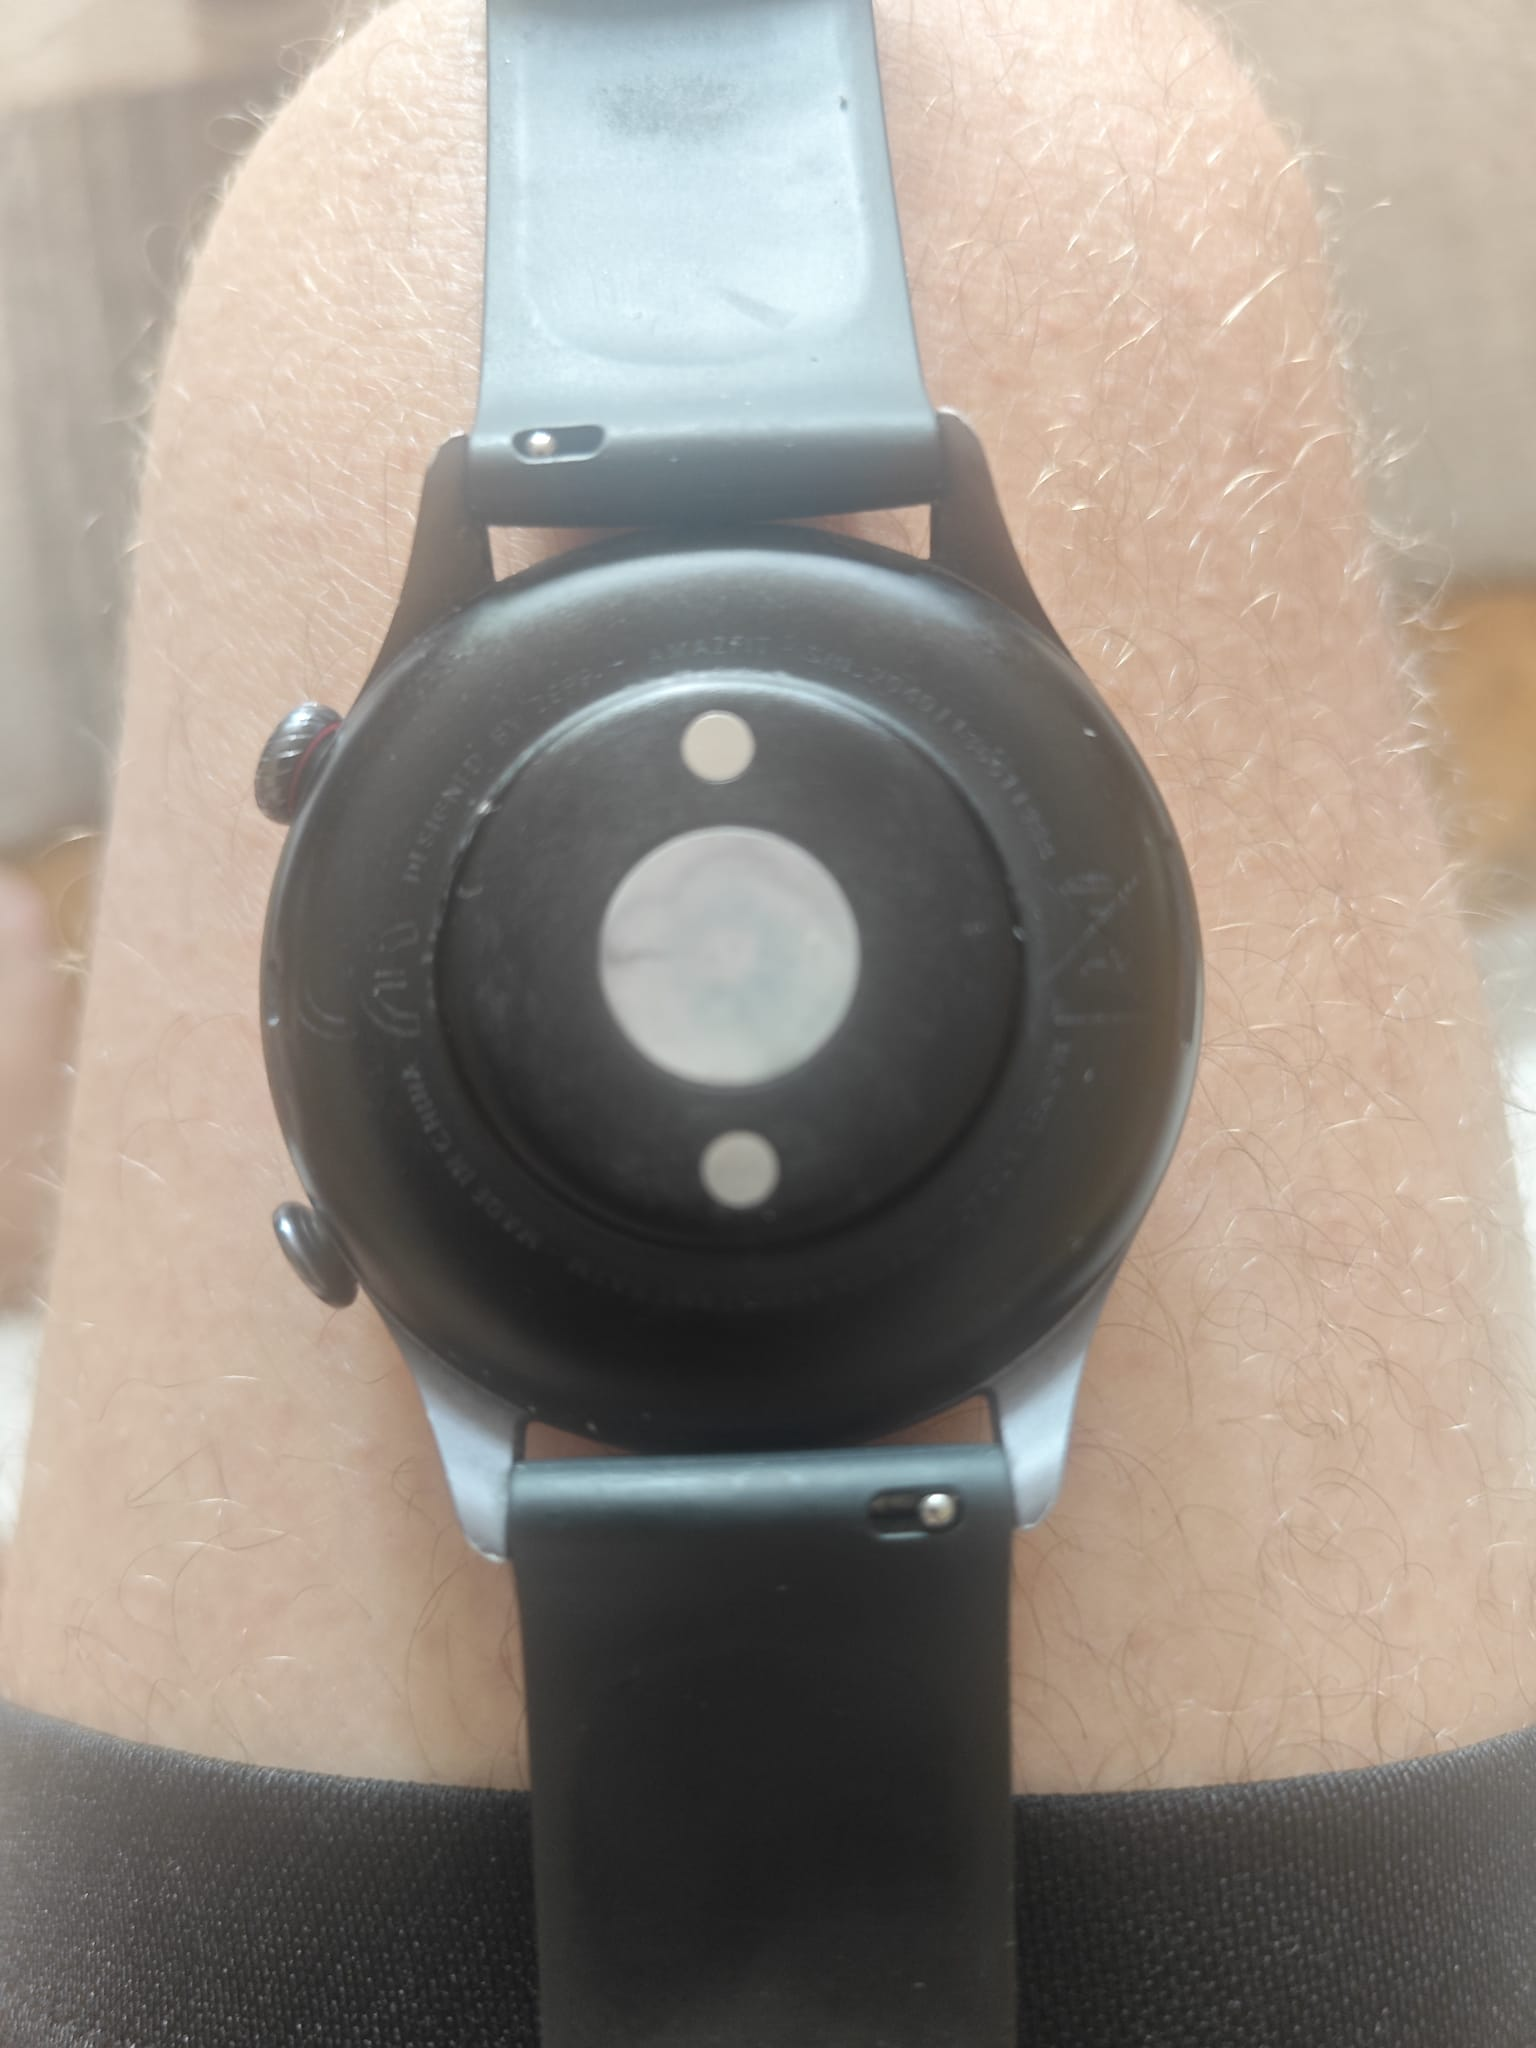
\includegraphics[width=\linewidth]{amazfit.jpeg}
			\caption{Amazfit GTR 3 Pro (wrist sensor)}
		\end{subfigure}\hfill
		\begin{subfigure}[b]{0.48\linewidth}
			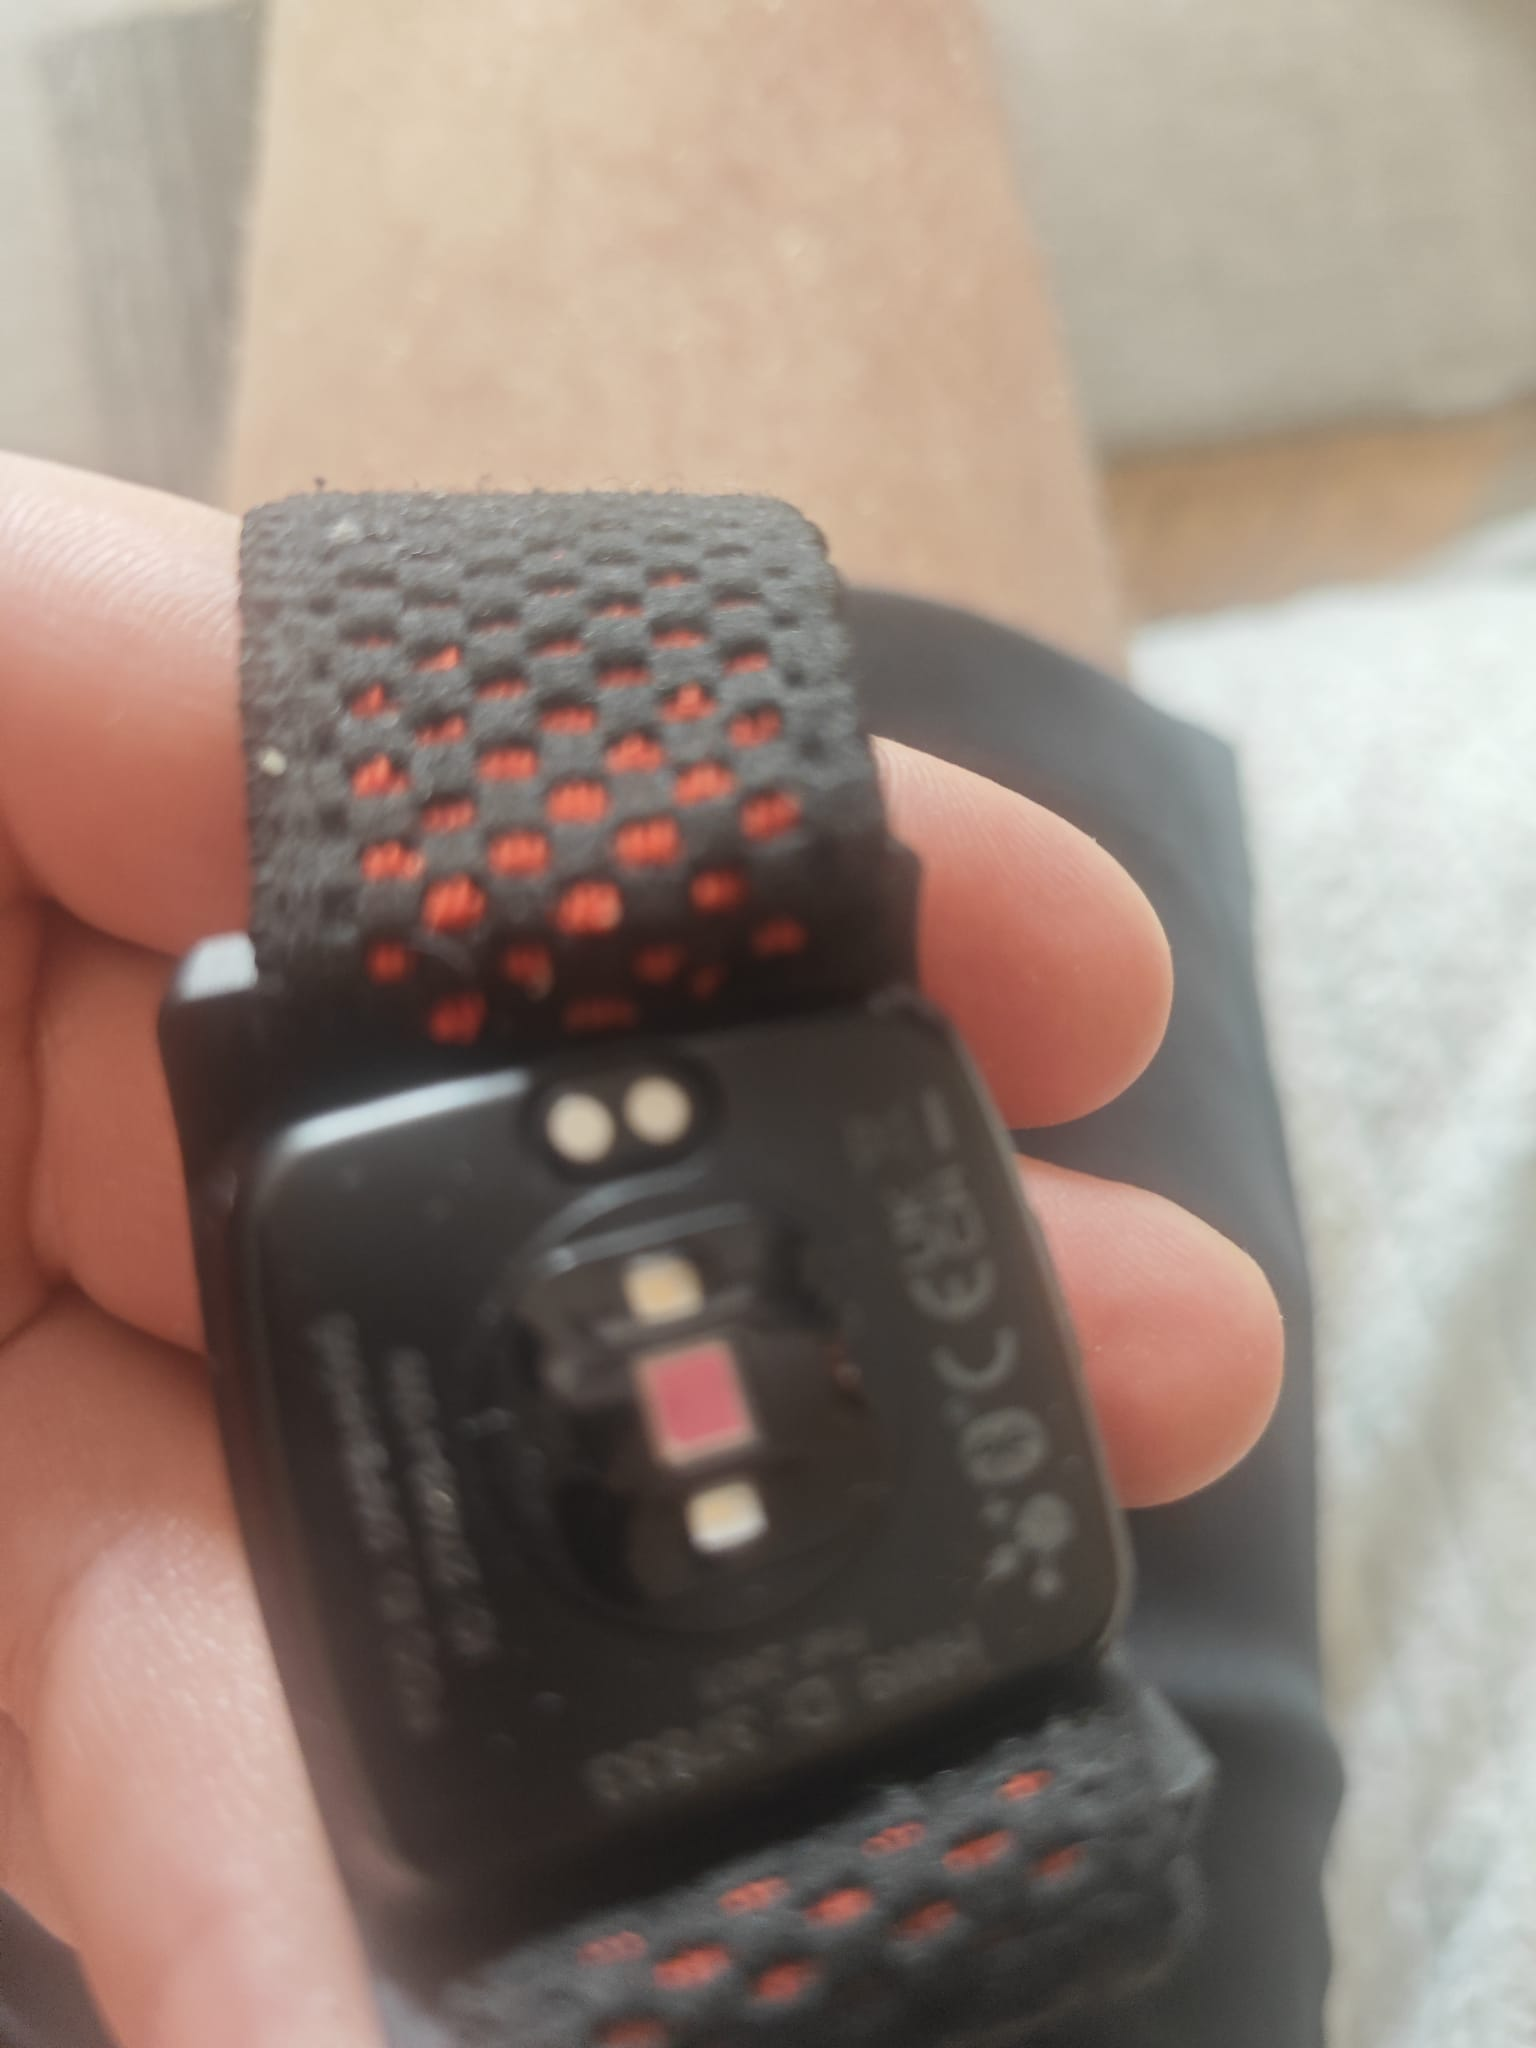
\includegraphics[width=\linewidth]{hw9.jpeg}
			\caption{Coospo HW9 (upper-arm sensor)}
		\end{subfigure}
		\caption{Visual comparison of the optical sensor arrays. (a) The
			over-4-year-old smartwatch shows a distinct round, milky-white
			discoloration and scratching directly over the PPG window. (b) The
			newer upper-arm array shows an intact, clear optical barrier.}
		\label{fig:devices}
	\end{figure}
	
	\paragraph{Agreement, not accuracy.} This study measures agreement
	between two consumer-grade optical sensors, neither of which is a
	clinically validated reference. We use the term \emph{accuracy}
	cautiously throughout; strictly speaking, our data support claims about
	\emph{cross-device agreement and relative data density}, not accuracy
	against ground truth. A stronger design would add a third, independently
	validated reference device (e.g., a chest-worn ECG strap) to establish
	true accuracy for both optical sensors.
	
	\paragraph{External validity.} All $N=6$ runs were performed by a single
	subject (intra-subject design). While this controls for
	inter-individual physiological variance, it means the reported
	statistics cannot be generalized to other runners, body compositions, or
	skin tones --- factors known to affect PPG signal quality. Future work
	should extend this protocol across multiple participants and, ideally,
	multiple device units per condition to separate placement effects from
	unit-specific wear. Geospatial tracking performed well overall in our
	data, with a study-wide mean spatial offset of $\approx$4.56\,m across
	all six runs (range 2.1--8.3\,m per-run mean, max.\ 30.5\,m;
	Figure~\ref{fig:gpsoffset}), though this combined average should not
	obscure the per-run variability visible in Table~\ref{tab:results}.
	
	\paragraph{Outlook: a derived metric for practitioners.} Independently
	of the device-comparison question above, amateur runners can make
	practical use of the acquired data via the Heart Rate Efficiency (HRE)
	metric (Equation~\ref{eq:hre}), defined as the quotient of velocity ($v$) and heart rate (HR):
	
	\begin{equation}
		\mathrm{HRE} = \frac{v}{\mathrm{HR}}
		\label{eq:hre}
	\end{equation}
	
	This metric has been proposed to scale with aerobic adaptation, offering
	a potentially more stable feedback signal than raw heart rate tracking
	alone \cite{Votyakov2025}. We flag it here only as a practical outlook
	rather than a validated contribution of this study: the formulation is
	currently supported by a single non-peer-reviewed preprint, and applying
	it would inherit all of the cross-device agreement limitations discussed
	above; we therefore recommend peer-reviewed replication before wider
	adoption.
	
	% ---------------------------------------------------------------
	\section{Conclusion}
	
	Within this single-subject, six-trial pilot, mean heart rate and
	geospatial tracking agreed closely between the wrist-worn Amazfit GTR~3~Pro
	and the upper-arm Coospo~HW9, but the aged wrist device showed
	substantial cardiac data loss (up to 74.6\% in the worst runs) and
	missed several transient load peaks that the upper-arm device captured.
	Because the two devices differ simultaneously in placement, hardware
	generation, and physical condition, we cannot attribute this gap to
	sensor placement alone; a confirmatory follow-up should use
	generation-matched devices (or the same model at both sites) together
	with an independent reference such as a chest-worn ECG strap, and should
	recruit enough trials or participants to reach adequate statistical
	power ($n\approx13$ trials indicated here). With those caveats, our data
	are consistent with upper-arm placement being a promising direction for
	high-density cardiac monitoring during intensive training, while
	wrist-worn tracking may remain adequate for steadier-state activity.
	
	\section*{Acknowledgements}
	
	The author used Gemini Pro (Google) and Mistral as AI-assisted writing
	tools during the preparation of this manuscript, primarily for language
	support including scientific English, grammar correction, wording, and
	stylistic refinement. All AI-assisted outputs were critically reviewed
	and edited by the author, who retains full responsibility for the
	content, accuracy, and integrity of the manuscript.
	
	\bibliographystyle{acmsiggraph}
	\bibliography{literatur}
	
\end{document}
